\documentclass[11pt,a4paper]{article}
\usepackage{amsmath}
\usepackage{amssymb}
\usepackage{fullpage}
\usepackage{graphicx}
\usepackage[colorlinks=true, linkcolor=blue]{hyperref}
\usepackage{makecell}

\newcommand{\argmin}{\operatornamewithlimits{arg\,min}}
\renewcommand{\arraystretch}{1.25} % line spacing in tabular

\begin{document}
\title{Improving Image Understanding with Concept Graph}
\author{Libo Yin\\The Australian National University}
\maketitle

\section{Introduction}

Document structure

\section{Background}

\section{The Original HEX Model}
\subsection{Structure}

The original HEX model \cite{deng2014large} is an extension of the baseline flat multiclass classification model. There are two types of multiclass classification: exclusive, where the classifier predicts exactly one out of all possible states to be true; and independent, where each state is predicted true or false independently. HEX finds a balance between these two ends of the spectrum. It models the Hierarchical and EXclusive relationship within the concept space of dataset, extended by their hypernyms, with a semantic graphical model. Each node in the HEX graph corresponds to a concept in the extended concept space being true or false. States of neighbouring nodes are constrained in that if $a$ is a hypernym of $b$, then is not allowed that $a=0,\ b=1$; and if $a$ and $b$ are exclusive, then they cannot both be true. HEX model classifies an image into a joint assignment of the state of nodes, corresponding to a hierarchy in the graphical model, that satisfies the above semantic consistency. A simple HEX graph is shown in \hyperref[fig:naive]{figure~\ref{fig:naive}}.
\begin{figure}[htbp]
\centering
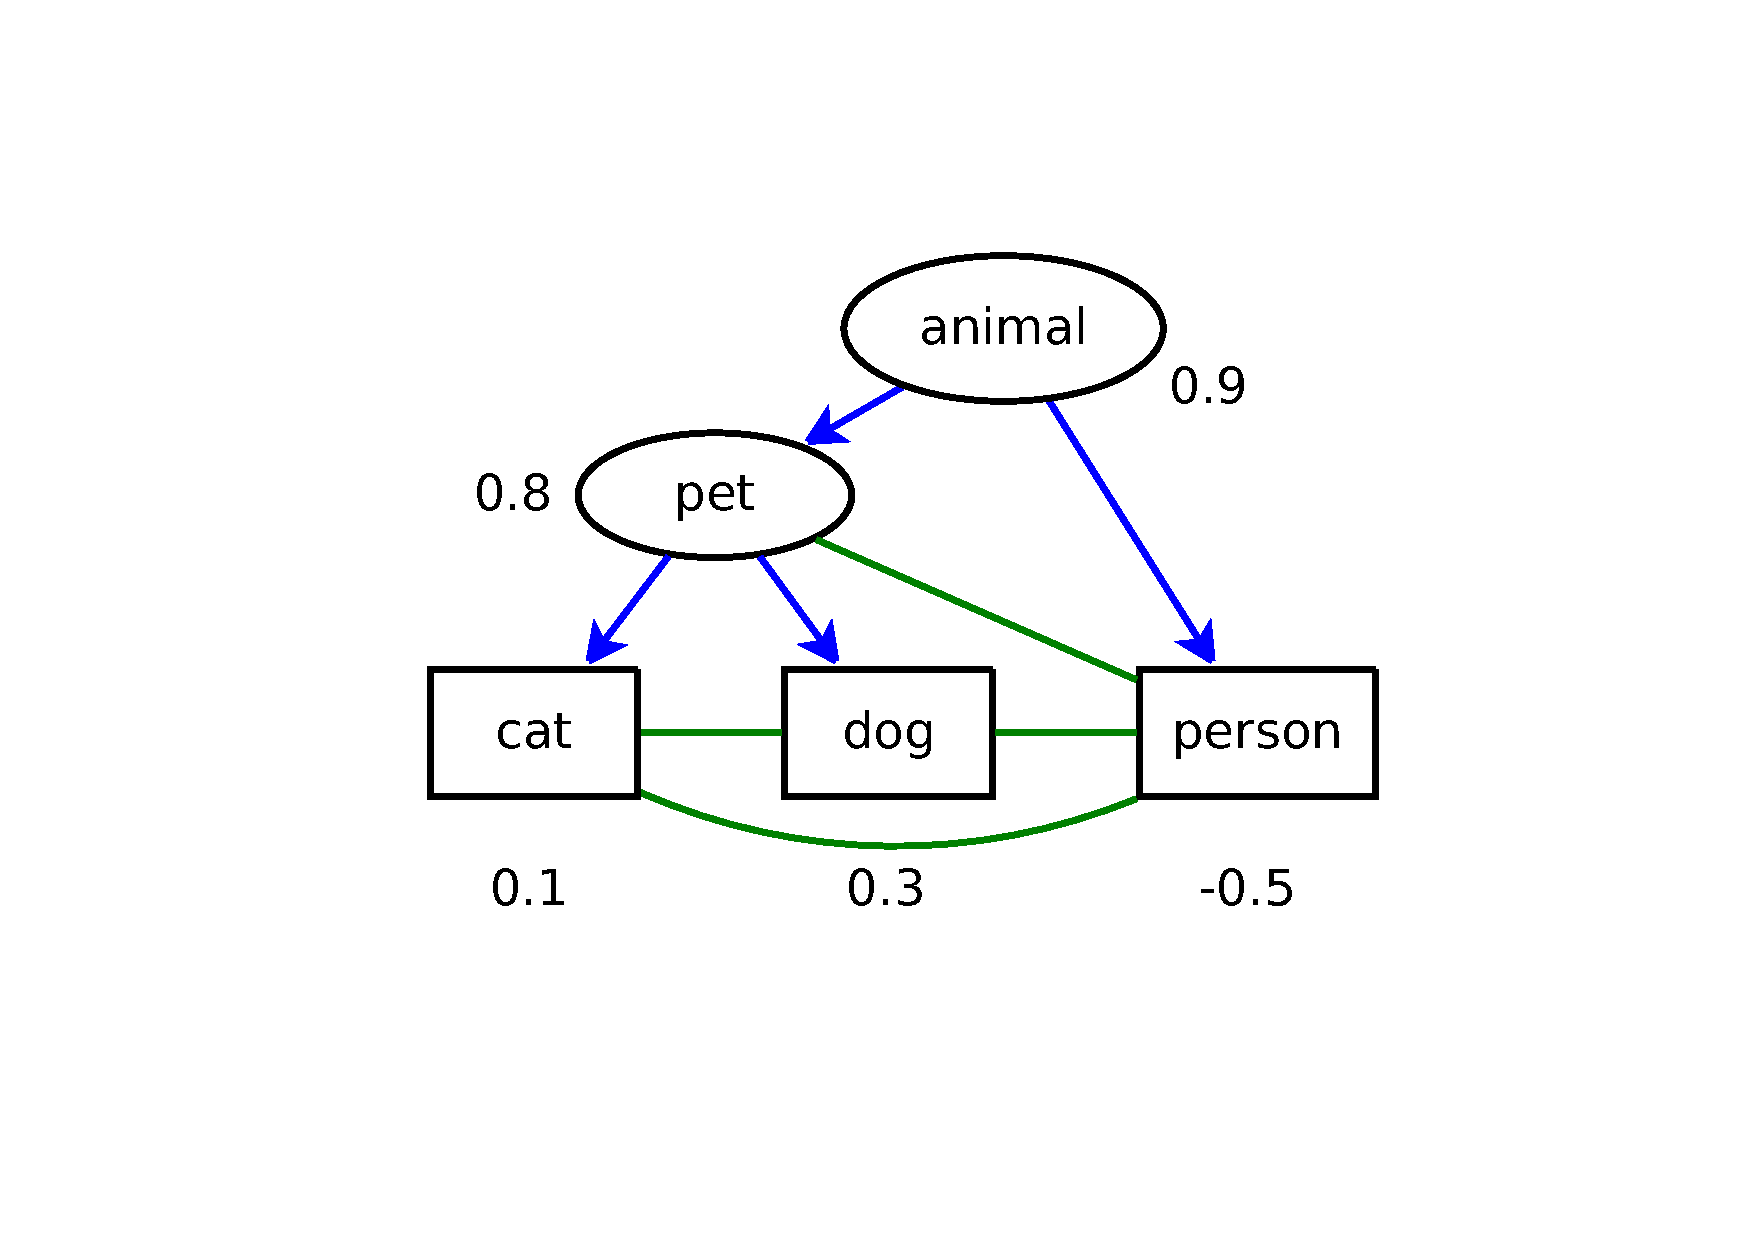
\includegraphics[scale=0.5]{naive.pdf}
\caption{A simple HEX graph with three nodes in the original concept space (in rectangles) and their hypernyms (in ellipsoids). Directed edges denote semantical subsumption: $(a\rightarrow b)$ if $a$ is a hypernym of $b$ according to WordNet; and undirected edges denote exclusion. Since exclusive relationship is not covered by WordNet, the exclusive subgraph is initialized greedily: two concepts are exclusive unless they share a common descendant in the hierarchical subgraph. Note that the hierarchical subgraph is in general a DAG rather than a tree; and it is not necessarily the case that all concepts in the original concept space are bottom-level nodes in the hierarchical subgraph. Values beside each nodes are to be used in \hyperref[tab:naive]{table~\ref{tab:naive}}.}
\label{fig:naive}
\end{figure}

Denoting the set of vertices by $V$, the set of hierarchical edges by $E_h$, and the set of exclusive edges by $E_e$, the joint assignment $y\in\{0,1\}^V$ can be defined as a conditional random field:
\begin{equation}
\tilde{p}(y|x)=\prod_{i\in V}\exp\{x_i\cdot I[y_i=1]\}I[y\text{ legal}]
\label{eqn:naive}
\end{equation}

where unary input $x_i$ is the confidence on concept $i$, predicted by an arbitrary underlying classifier\footnote{According to \cite{deng2014large}. It shall be explained in \hyperref[sec:observ]{section~\ref{sec:observ}} that the choice of underlying unary classifier is actually not arbitrary.}. Local semantic constraints on hierarchical and exclusive edges is formalised by:
\begin{equation}
I[y\text{ legal}]=\prod_{(v_i,v_j)\in E_h}I[(y_i,y_j)\neq(0,1)]\prod_{(v_i,v_j)\in E_e}I[(y_i,y_j)\neq(1,1)]
\label{eqn:legal}
\end{equation}

Thanks to these semantic constraints, the state space of a HEX graph, i.e.\ the set of all legal joint assignments, is significantly smaller than the state space of independent multiclass classification on the same concept space. For example, with local confidence given beside each node in \hyperref[fig:naive]{figure~\ref{fig:naive}}, the valid assignments of the HEX graph and their respective potentials are shown in \hyperref[tab:naive]{table~\ref{tab:naive}}.

\begin{table}[htbp]
\centering
\begin{tabular}{r|l}
assignment & $\tilde{p}(y|x)$\\
\hline
$\varnothing$ & $\exp(0)$\\
\{animal\} & $\exp(0.9)$\\
\{animal, pet\} & $\exp(0.9+0.8)$\\
\{animal, person\} & $\exp(0.9-0.5)$\\
\{animal, pet, cat\} & $\exp(0.9+0.8+0.1)$\\
\{animal, pet, dog\} & $\exp(0.9+0.8+0.5)$\\
\{animal, pet, dog, Husky\} & $\exp(0.9+0.8+0.5-0.1)$\\
\{animal, pet, dog, Labrador\} & $\exp(0.9+0.8+0.5+0.3)$
\end{tabular}
\caption{The extended state space, i.e.\ all valid assignments of the HEX graph in \hyperref[fig:naive]{figure~\ref{fig:naive}}, and their respective potentials. In this example, the most likely joint assignment is \{animal, pet, dog, Labrador\}. The softmax baseline classifier, in the language of HEX, classifies to the original state space: \{animal, pet, cat\}, \{animal, pet, dog\}, \{animal, pet, dog, Husky\}, \{animal, pet, dog, Labrador\}, and \{animal, person\}.}
\label{tab:naive}
\end{table}

Finally, an important assumption of \cite{deng2014large} is that mechanical Turks tend to label an image to more abstract concepts. For example, an image of a yellow Labrador is more likely to be labelled to ``dog'' than ``Labrador''. Such realistic labelling behaviour is modelled by randomly relabelling images to their immediate parents. A major task of the HEX model is to make accurate predictions when the relabelling rate is high.

\subsection{Observations}
\label{sec:observ}

Note that a valid assignment does not have to have an active node in the original concept space. (Actually, it does not have to have an active node at all, as $\varnothing$ is a valid joint assignment according to \hyperref[eqn:legal]{(\ref{eqn:legal})}.) This allows an image to be classified to a joint assignment in which all active concepts are abstract. For example, in \hyperref[fig:naive]{figure~\ref{fig:naive}}, to \{$\varnothing$\}, \{animal\}, or \{animal, pet\}. This is by no doubt a desirable feature for deployment. However, since all images are labelled in the original concept space, classifying to the extended concept space makes performance evaluation troublesome. While this issue is not addressed in \cite{deng2014large}, the evaluation strategy used for this work will be discussed in \hyperref[sec:exp1]{section~\ref{sec:exp1}}.

Also note that in \hyperref[tab:naive]{table~\ref{tab:naive}}, the competition between assignment \{animal, pet, dog, Husky\} and \{animal, pet, dog, Labrador\} depends entirely on the confidence of node ``Husky'' and ``Labrador''. However, to discriminate between \{animal, pet, dog, Husky\} and \{animal, person\} requires examining the confidence along different paths. From this example it is clear that, in the testing stage, confidence is passed down the hierarchy from more abstract concepts to more concrete ones. The other side of the same coin is that, during the training stage of the underlying unary classifier, a node corresponding to abstract concepts receive all training data of its children. This can be seen as confidence being passed up in the hierarchy. Such bidirectional propagation of confidence explains the advantage of the HEX model under the realistic labelling assumption. Note that the exclusive subgraph does not take part in the propagation of confidence.

The third observation is a combined consequence of the greedy exclusion setup, as discussed under \hyperref[fig:naive]{figure~\ref{fig:naive}}, and the greedy nature of the potential function \hyperref[eqn:naive]{(\ref{eqn:naive})}. The prerequisite for the original HEX model is that the decision boundary of $x_i$ is zero for all $i$: A unary prediction above zero gives support to a node being active (true), whereas a unary prediction below zero gives support to that node being inactive (false). In \cite{deng2014large} this is not a problem, as a convolutional neural network \cite{krizhevsky2012imagenet} is used as the underlying unary classifier; and a neural network can learn its decision boundary from training data. However, if a probabilistic classifier is used, in which case $x_i\in[0,1]$ and the decision boudary is 0.5, then it is guaranteed that a bottom-level node will be activated (see \hyperref[sec:fail]{appendix~\ref{sec:fail}} for proof). This means that the effective state space size of the HEX graph is reduced to the number of bottom-level nodes, which is no larger than the original state space size. This defeats the purpose of HEX, although a smaller state space means faster inference and higher accuracy.

Finally, listed below are two less important observations:
\begin{enumerate}
\item There are no learnable variables in this CRF. In other words, all learning is performed in the underlying unary classifier.
\item Mathematically, CRF requires $\forall y:\tilde{p}(y|x)>0$. However, computationally, assigning zero to $\tilde{p}(y|x)$ can be interpreted as assigning an infinitesimal value. Therefore, the above definition is computationally a legitimate CRF.
\end{enumerate}

\subsection{Problems}
\label{sec:problem}

\begin{figure}[htbp]
\centering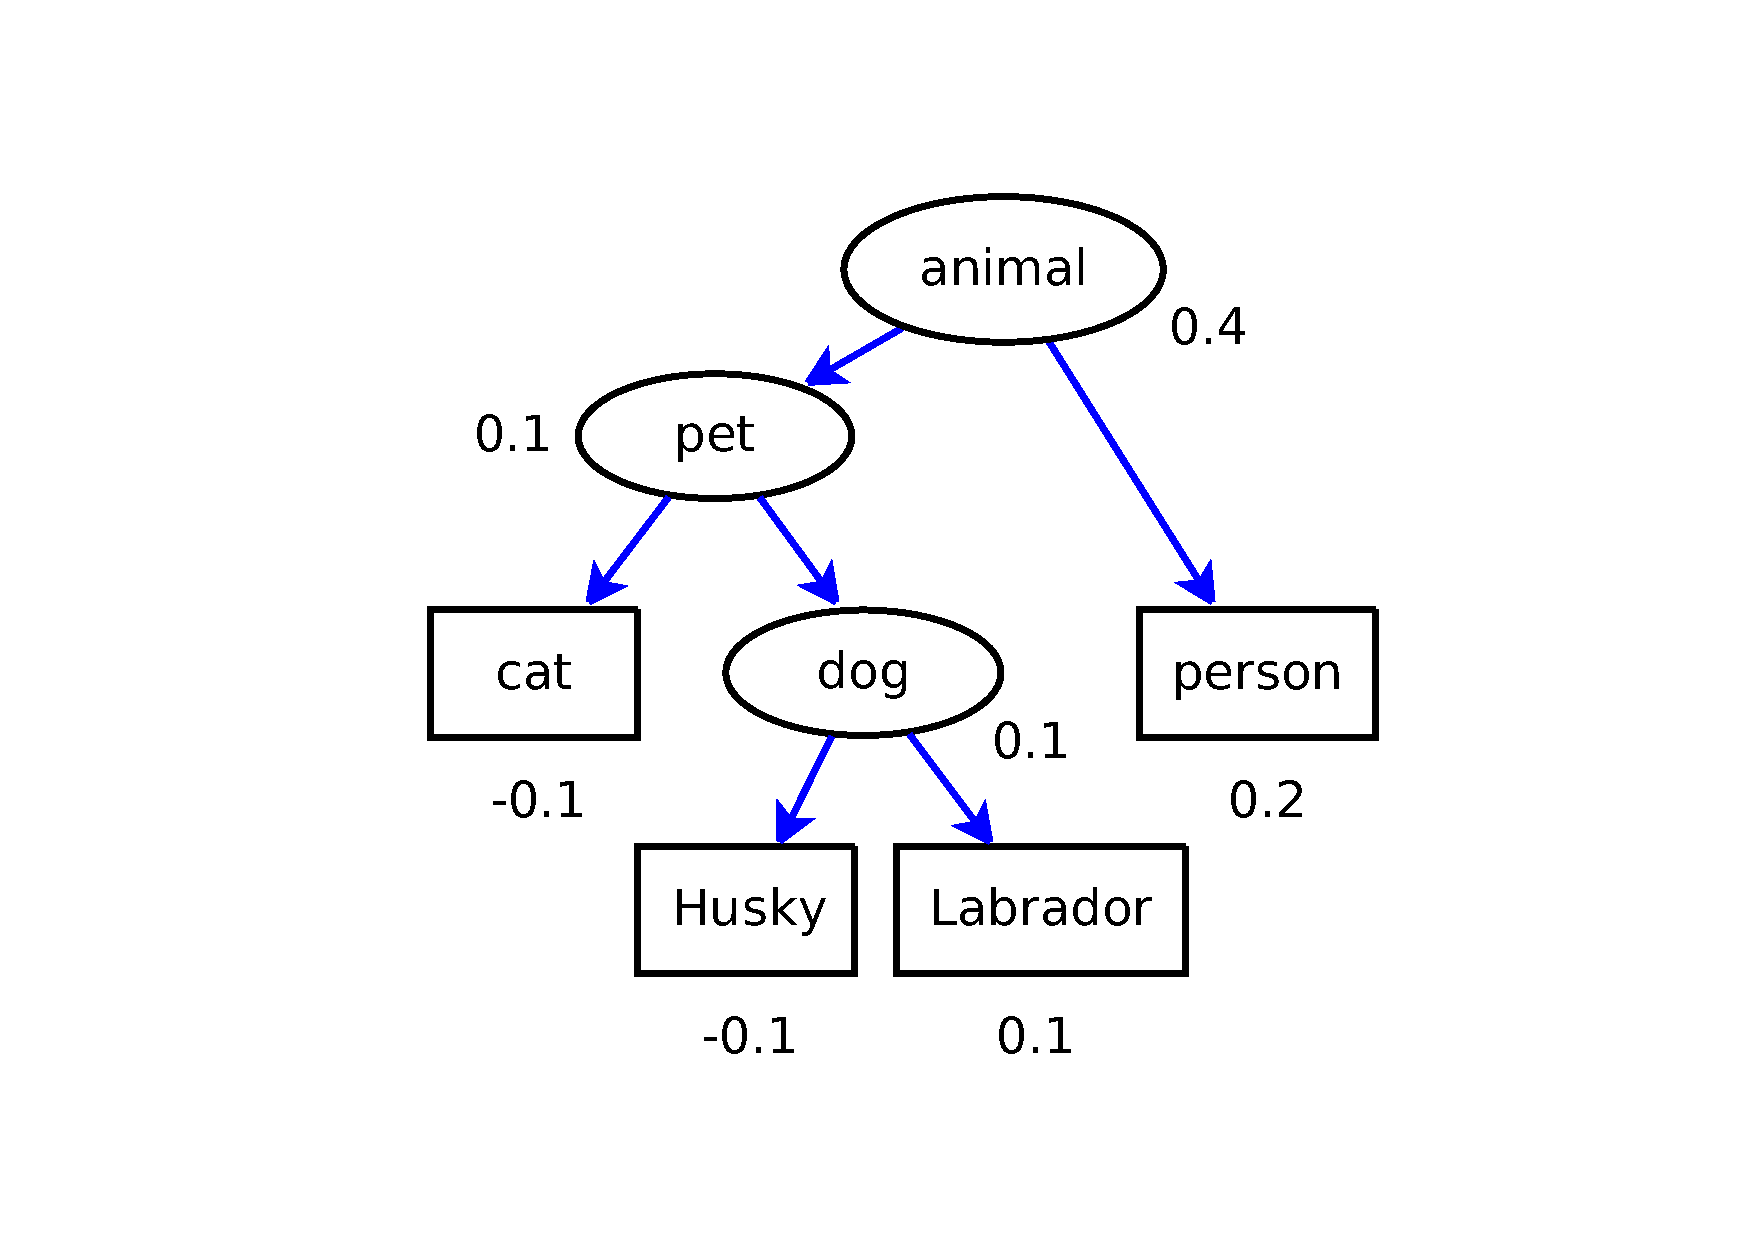
\includegraphics[scale=0.5]{depth.pdf}
\caption{Where an assignment with more active nodes of lower confidence wins over an assignment with fewer active nodes of higher confidence. Exclusive edges are not drawn, as they do not carry further information once the state space has been calculated.}
\label{fig:depth}
\end{figure}

Consider the situation illustrated in \hyperref[fig:depth]{figure~\ref{fig:depth}}. Following the same logic as \hyperref[tab:naive]{table~\ref{tab:naive}}, the original HEX model predicts \{animal, pet, dog, Labrador\}. However, this is a result of more active nodes rather than active nodes of higher confidence. Intuitively, \{animal, person\} seems a more reasonable prediction. In addition, the two aforementioned assignments are only separated by 0.1 in log unnormalised potential. It will be desirable if the model can make a prediction that is further from the decision boundary by taking into account the confidence of other nodes, especially those with unary predictions far from the decision boundary.

The second problem is a combined consequence of the realistic labelling assumption and using an independent multiclass classifier as the underlying unary classifier. When the relabelling rate is high, most images are relabelled to their immediate parents. This means that for each concept $X$, most instances of $X$ are correctly labelled to all its ancestors, but incorrectly labelled ``NOT $X$''. This create a highly unbalanced and internally inconsistent dataset. In such case, for images of $X$, the unary predictions will highly likely be ``NOT $X$''. (This hypothesis will be confirmed in \hyperref[sec:exp1]{section~\ref{sec:exp1}}.) This problem becomes more serious with small training dataset \cite{he2009learning}. The original HEX model does not cope with such situation, as the potential function \hyperref[eqn:naive]{(\ref{eqn:naive})} deactivates a bottom-level node as long as its unary confidence is below the decision boundary.

\section{Reimplementation}
\subsection{Dataset}
\label{sec:data}

The original HEX model is reimplemented as the baseline of this work. While \cite{deng2014large} used ILSVRC 2012 dataset for its rich structure in the label space, this work employs PASCAL VOC 2012 \cite{pascal-voc-2012} for its simplicity. The complete hierarchical subgraph is shown in \hyperref[fig:hex]{figure~\ref{fig:hex}}. Note that the two datasets are designed for different tasks: ILSVRC is an exclusive multiclass classification problem, whereas PASCAL is an independent multiclass classification problem. To adapt to ILSVRC task 1, the train+val dataset of PASCAL is filtered through the following criteria:
\begin{enumerate}
\item If there is only one annotated object in the image, the image is labelled to that object.
\item If the largest annotated object in the image is more than twice as large as the second largest one, the image is labelled to its dominating object.
\end{enumerate}

Another major difference between ImageNet and PASCAL is that the former one is a balanced dataset, while the latter is highly unbalanced. For example, after filtering, there are 5,324 images labelled as ``person'', whereas the second most frequent label ``dog'' has only 817 instances. To rebalance the dataset, 950 images of ``person'' are subsampled from the filtered dataset.  After preprocessing, the dataset contains 8,473 images in total. These images are then split 3:1:1 into train/validation/test set. The distribution of images across labels is illustrated in \hyperref[fig:distro]{figure~\ref{fig:distro}}.
\begin{figure}[htbp]
\centering
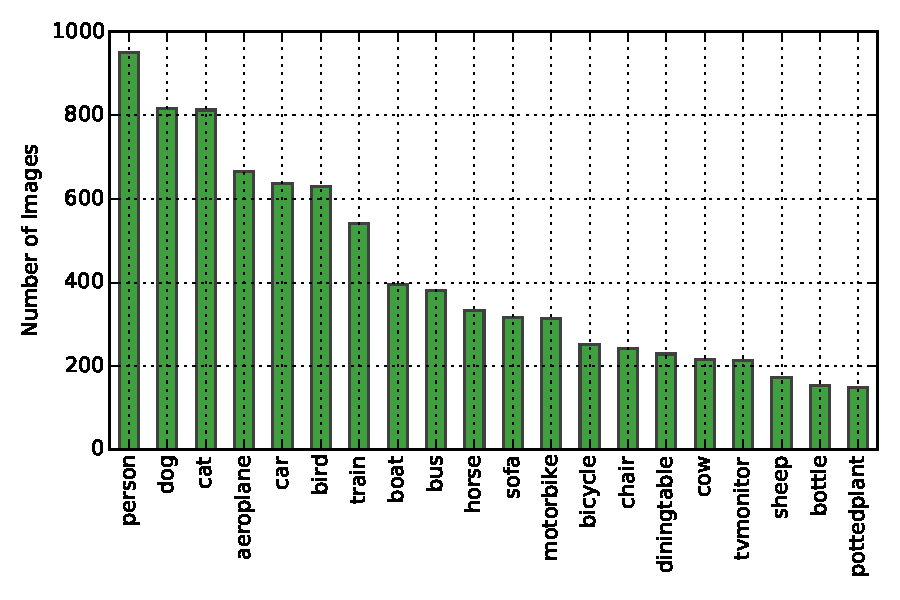
\includegraphics[scale=0.8]{distro.pdf}
\caption{Distribution of images according to labels, after preprocessing.}
\label{fig:distro}
\end{figure}
\begin{figure}[p]
\centering
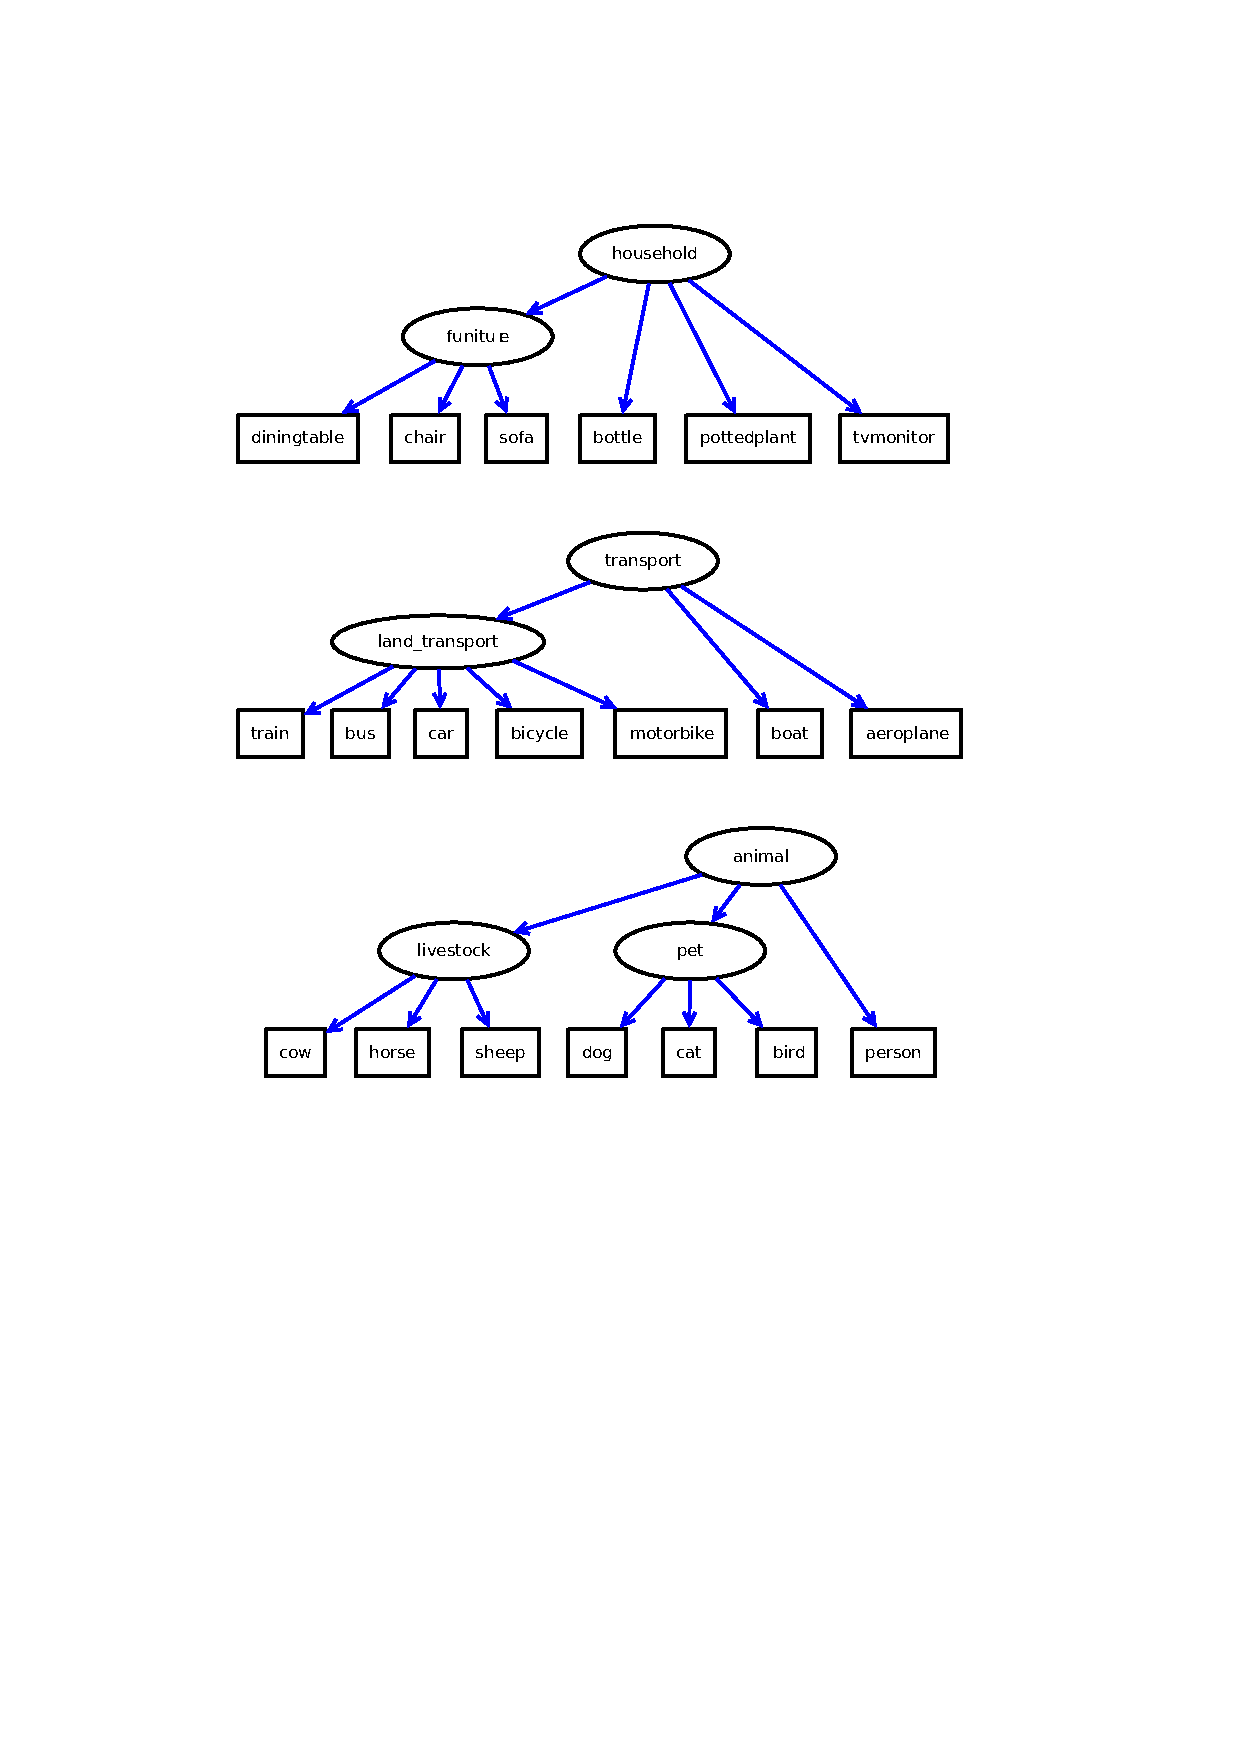
\includegraphics[scale=1.1]{full.pdf}
\caption{The PASCAL dataset has 20 concepts, as shown in rectangles. In this work, these concepts are extended by 7 of their hypernyms, creating a forest of three trees with 27 nodes and 24 hierarchical edges. Exclusive edges are not drawn since they can be implied by the hierarchical subgraph. The state space of this HEX graph has size 28. In comparison, the HEX graph in \cite{deng2014large} contains 1000 nodes corresponding to the original concept space, and 820 nodes corresponding to their hypernyms. Note that there is no hierarchical relationship within the original concept space.}
\label{fig:hex}
\end{figure}

\subsection{Algorithms}

For consistency with \cite{deng2014large}, the underlying unary classifier is based on \cite{krizhevsky2012imagenet} instead of the current state-of-the-art \cite{simonyan2014very}. The CNN, originally trained on ImageNet, is fine-tuned as an independent multiclass classifier on PASCAL, where each image is projected to a 27-dimensional vector. Note that since the original HEX model has no learning part, it was built as a layer into the CNN, achieving end-to-end learning. In this work, CNN and CRF are implemented separately, such that multiple variants of the HEX model can be tested with the same underlying unary classifier. For details of CNN setup, refer to \hyperref[sec:setup]{appendix~\ref{sec:setup}}.

A simpler concept space also lead to the change of inference algorithm. In \cite{deng2014large}, inference is performed by MAP loopy belief propagation on the HEX graph, where the local state space of each clique is constrained by semantic restrictions (see \hyperref[sec:scale]{section~\ref{sec:scale}} for details). In this work, due to the small concept space of dataset, the inference is performed by calculating the potential function directly for each state in the global state space.

Finally, to guarantee that the benefit of the HEX model is consistent regardless of the underlying unary classifier, different variants of the HEX model are also paired with SVM as the underlying unary classifier. An array of 27 SVMs is trained, each corresponding to a node in the HEX graph. The SVM array accepts the output of the last-but-one layer of \cite{krizhevsky2012imagenet} as input, assuming that 4,096 neurons provide sufficiently diverse and accurate feature responses \emph{without} fine-tuning on the PASCAL dataset. The SVM array predicts distance to decision boundaries, corresponding to raw CNN output without sigmoid transformation. For details of SVM setup, refer to \hyperref[sec:setup]{appendix~\ref{sec:setup}}.

\subsection{Experiments}
\label{sec:exp1}

In this work, accuracy is tested both in the extended state space and in the original state space, emphasizing on the former one. Testing in the original state space is achieved by limiting the legal state space to assignments with an active bottom-level node in the hierarchical subgraph; or in case of flat classification baseline, to the original concept space. Note that this is only valid for datasets where all concepts in the original concept space are bottom-level nodes in the hierarchical subgraph.

The empirical test result of \cite{deng2014large} and the reimplemented system are compared in \hyperref[tab:original]{table~\ref{tab:original}}. Due to the size of PASCAL dataset, relabelling rate of 95\% is not attempted in this work. Observations on the experimental results are listed as follows:
\begin{enumerate}
\item Regardless of implementation and inference algorithm, the accuracy drops as the relabelling rate grows. This is within expectation.
\item In the extended state space, independent classification baseline by itself tend to have the lowest accuracy. However, in the original state space, the accuracy of independent classification can sometimes beat the softmax baseline. This is a clear sign that nodes corresponding to abstract concepts in the HEX graph receive higher confidence than bottom-level nodes. With the propagation of confidence discussed in \hyperref[sec:observ]{section~\ref{sec:observ}}, the HEX model is able to recover classification information on bottom-level nodes to a similar level as the softmax baseline.
\item In \cite{deng2014large}, the original HEX model managed to beat the softmax baseline under all relabelling rates (except for 0\%, on which only the accuracy of softmax baseline is provided). However, with the reimplemented system in the extended state space, the accuracy of HEX falls below the softmax baseline. In addition, as the relabelling rate grows, the accuracy of the reimplemented system drops much faster than in \cite{deng2014large}. This is a clear sign of insufficient confidence on bottom-level concepts, as discussed in \hyperref[sec:problem]{section~\ref{sec:problem}}. This problem is also inspected in \hyperref[tab:resp]{table~\ref{tab:resp}}.
\end{enumerate}

\begin{table}[htbp]
\centering
\begin{tabular}{r|c|c|c|c}
 & 0\% & 50\% & 90\% & 95\%\\
\hline
Softmax     & 0.626(0.843) & 0.564(0.796) & 0.529(0.772) & 0.508(0.760)\\
Independent & N/A          & 0.210(0.452) & 0.093(0.272) & 0.056(0.172)\\
HEX         & N/A          & 0.582(0.808) & 0.553(0.794) & 0.524(0.772)\\
\hline
Softmax     & 0.669(0.906) & 0.332(0.816) & 0.007(0.738) & N/A\\
Independent & 0.171(0.863) & 0.004(0.811) & 0.000(0.407) & N/A\\
HEX         & 0.657(0.893) & 0.318(0.869) & 0.000(0.838) & N/A\\
\hline
Softmax     & 0.673(0.906) & 0.622(0.896) & 0.561(0.871) & N/A\\
Independent & 0.726(0.937) & 0.673(0.930) & 0.323(0.640) & N/A\\
HEX         & 0.720(0.894) & 0.685(0.888) & 0.502(0.872) & N/A
\end{tabular}
\caption{Comparison of empirical test result in \cite{deng2014large} (top) with the reimplemented system (middle: extended concept space; bottom: original concept space). Performance is reported in accuracy, with top-5 accuracy in the bracket. The softmax baseline is obtained by training a CNN that maps an image to exactly one node in the HEX graph, discarding all hierarchical information. The independent classification baseline is obtained by classifying to the concept with the highest unary confidence.}
\label{tab:original}
\end{table}

\begin{table}[htbp]
\centering
\begin{tabular}{r|c|c|c}
 & 0\% & 50\% & 90\%\\
\hline
diningtable & $0.4285\pm0.3011$ & $0.2490\pm0.2288$ & $0.0108\pm0.0116$\\
furniture   & $0.6976\pm0.3298$ & $0.7524\pm0.2784$ & $0.7330\pm0.3065$\\
household   & $0.8431\pm0.2729$ & $0.8598\pm0.2490$ & $0.8590\pm0.2494$\\
\hline
dog         & $0.7517\pm0.3424$ & $0.4533\pm0.2970$ & $0.0222\pm0.0209$\\
pet         & $0.7971\pm0.3271$ & $0.7828\pm0.3327$ & $0.7832\pm0.3287$\\
animal      & $0.9004\pm0.2301$ & $0.9005\pm0.2290$ & $0.8999\pm0.2322$
\end{tabular}
\caption{Under different relabelling rates, with fully trained CNN, the mean and standard deviation of sigmoid-transformed response on validation images labelled ``diningtable'' (upper) and ``dog'' (lower). Note that ``household'' is a hypernym of ``furniture'', which is further a hypernym of ``diningtable''; and ``animal'' is a hypernym of ``pet'', which is further a hypernym of ``dog''. With 490 instances in the training set, label ``dog'' is a frequent concept, whereas rare concept ``diningtable'' has 137 instances in the training set. Clearly, the unary response on abstract concepts are not affected by the relabelling rate, yet on bottom-level concepts, the confidence drops to below the decision boundary.  This experiment also shows that CNN learns highly abstract concepts accurately, even for concepts without visual clues such as ``household''.}
\label{tab:resp}
\end{table}

\section{Improvements}
\subsection{Algorithms}

Based on the original HEX model, this work delivers improvements in three stages, where each stage is built on top of the previous one. The high-level goal of improvements is stated as follows: With little confidence on bottom-level nodes, the classifier should attempt to classify to an assignment with an active bottom-level concept. However, in case the classifier is not confident enough to do so, it should be allowed to predict to a joint assignment in the extended state space.

In the first stage, the confidence on inactive nodes are taken into consideration, in addition to active ones. The resulting unnormalised potential function is shown as follows:
\begin{equation}
\tilde{p}(y|x)=\prod_{i\in V}\exp\{x_iI[y_i=1]+(1-x_i)I[y_i=0]\}I[y\text{ legal}]
\label{eqn:pn1}
\end{equation}

where $x_i$ denotes the confidence of node $i$ being true, and $1-x_i$ for being false. This requires the range of the unary prediction to be within $[0,1]$, and the decision boundary to be 0.5. To achieve this, unary predictions from the underlying classifier are normalised with the sigmoid function.

Theoretically, stage 1 fix should benefit in two aspects: First, the potential function considers the same number of nodes for every legal joint assignment, therefore fixing the unnormalised depth problem discussed in \hyperref[sec:problem]{section~\ref{sec:problem}}. Second, the potential function is able to refer to the confidence of inactive nodes, hence benefiting from those that are far from the decision boundary. However, a massage on \hyperref[eqn:pn1]{(\ref{eqn:pn1})} shows that it is not far from the original potential function \hyperref[eqn:naive]{(\ref{eqn:naive})}:
\begin{align}
\tilde{p}(y|x)&=\prod_{i\in V}\exp\{x_i\cdot I[y_i=1]+(1-x_i)(1-I[y_i=1])\}I[y\text{ legal}]\nonumber\\
&=\prod_{i\in V}\exp\{(2x_i-1)I[y_i=1]+(1-x_i)\}I[y\text{ legal}]\nonumber\\
&=\tilde{p}(\varnothing|x)\prod_{i\in V}\exp\{(2x_i-1)I[y_i=1]\}I[y\text{ legal}]
\label{eqn:pn2}
\end{align}

where $\tilde{p}(\varnothing|x)$ denotes the unnormalised potential of assignment $\varnothing$. Since $\tilde{p}(\varnothing|x)$ only depends on $x$, it can be absorbed into the partition function $\frac{1}{Z(x)}$. Also, $\exp\{(2x_i-1)I[y_i=1]\}$ does not affect the rank of $\tilde{p}(y|x)$ for all $y$. Therefore, the difference between \hyperref[eqn:naive]{(\ref{eqn:naive})} and \hyperref[eqn:pn1]{(\ref{eqn:pn1})} is no more than the sigmoid transformation.

In the second stage, pairwise terms are added to the potential function. This fix is a remedy to the low confidence problem on bottom-level nodes when the relabelling rate is high, by exploiting the fact that the confidence on the immediate parents of bottom-level nodes are not affected by the relabelling rate. In addition, two regularisation constants are added to the potential function, such that the contributions from unary and pairwise terms are balanced. The resulting unnormalised potential function is shown as follows:
\begin{align}
p(y|x)=\frac{1}{Z(x)}&\exp\left\{\frac{1}{|V|}\sum_{i\in V}x_i\cdot I[y_i=1]+(1-x_i)\cdot I[y_i=0]\right\}\nonumber\\
\cdot&\exp\left\{\frac{1}{|E_h|}\sum_{(i,j)\in E_h}x_ix_j\cdot I[y_i=y_j=1]\right\}\cdot I[y\text{ legal}]
\end{align}

In the third stage, a weighting factor is added to each unary and pairwise term. This weighting factor is learned form all images labelled to bottom-level concepts in the training dataset. Note that such training scheme cannot cover concepts from the original concept space that are not bottom-level nodes in the HEX graph, as it is not possible to distinguish between images that are correctly labelled to that concept, or images that are relabelled to its immediate parents. For example, in \hyperref[fig:naive]{figure~\ref{fig:naive}}, only images labelled to ``cat'', ``Husky'', ``Labrador'', and ``person'' are used to train the CRF, while images labelled to ``dog'' are discarded, even though ``dog'' is within the original concept space. The resulting normalised potential function is shown as follows:
\begin{align}
p_\theta(y|x)=\frac{1}{Z(x)}&\exp\left\{\frac{1}{|V|}\sum_{i\in V}w_i\big(x_i\cdot I[y_i=1]+(1-x_i)\cdot I[y_i=0]\big)\right\}\nonumber\\
\cdot&\exp\left\{\frac{1}{|E_h|}\sum_{(i,j)\in E_h}t_{ij}\cdot x_ix_j\cdot I[y_i=y_j=1]\right\}\cdot I[y\text{ legal}]
\end{align}

where $\theta$ is the concatenation of $\{\forall i\in V:w_i\}$ and $\{\forall(i,j)\in E_h:t_{ij}\}$. $\theta$ is selected by optimising for log-likelihood:
\begin{equation}
\theta=\argmin_\theta\left\{-\frac{C}{N}\log\prod_{(x,y)\in D}p_\theta(y|x)+\frac{1}{2}\|\theta\|^2\right\}
\end{equation}

where the weighting of regularisation term $\frac{1}{2}\|\theta\|^2$ is controlled by $C$, a constant chosen by cross-validation. In this work, $C=1000$. The gradient is calculated piecewisely:
\begin{align}
\nabla_\theta\log\prod_{(x,y)\in D}p_\theta(y|x)&=\begin{bmatrix}
\nabla_w\log\prod_{(x,y)\in D}p_\theta(y|x)\\ 
\nabla_t\log\prod_{(x,y)\in D}p_\theta(y|x)
\end{bmatrix}\nonumber\\
&=\begin{bmatrix}
\sum_{(x,y)\in D}\nabla_w\log p_\theta(y|x)\\ 
\sum_{(x,y)\in D}\nabla_t\log p_\theta(y|x)
\end{bmatrix}
\label{eqn:nablatheta}
\end{align}

The log-likelihood in \hyperref[eqn:nablatheta]{(\ref{eqn:nablatheta})} is expanded as follows:
\begin{align}
\log p_\theta(y|x)&=\frac{1}{|V|}\sum_{i\in V}w_i(x_i\cdot I[y_i=1]+(1-x_i)\cdot I[y_i=0])\nonumber\\
&\quad+\frac{1}{|E_h|}\sum_{(i,j)\in E_h}t_{ij}\cdot x_ix_j\cdot I[y_i=y_j=1]-\log\sum_{\hat{y}}\tilde{p}_\theta(\hat{y}|x)
\end{align}

Therefore, the gradient in the first line of \hyperref[eqn:nablatheta]{(\ref{eqn:nablatheta})} is calculated as:
\begin{align}
\nabla_w\log p_\theta(y|x)&=\frac{1}{|V|}\Big[x_i\cdot I[y_i=1]+(1-x_i)\cdot I[y_i=0]\Big]_{i\in V}-\nabla_w\log\sum_{\hat{y}}\tilde{p}_\theta(\hat{y}|x)\nonumber\\
&\quad\text{define }\phi_u(x,y)=\frac{1}{|V|}\Big[x_i\cdot I[y_i=1]+(1-x_i)\cdot I[y_i=0]\Big]_{i\in V}\nonumber\\
&=\phi_u(x,y)-\sum_{\hat{y}}p_\theta(\hat{y}|x)\cdot\phi_u(x,\hat{y})
\label{eqn:nablaw}
\end{align}

where the gradient of the partition function in \hyperref[eqn:nablaw]{(\ref{eqn:nablaw})} is calculated as:
\begin{align}
\nabla_w\log\sum_{\hat{y}}\tilde{p}_\theta(\hat{y}|x)&=\frac{1}{\sum_{\hat{y}}\tilde{p}_\theta(\hat{y}|x)}\nabla_w\sum_{\hat{y}}\tilde{p}_\theta(\hat{y}|x)\nonumber\\
&=\frac{1}{Z(x)}\sum_{\hat{y}}\nabla_w\exp\left\{\frac{1}{|V|}\sum_{i\in V}w_i\big(x_i\cdot I[y_i=1]+(1-x_i)\cdot I[y_i=0]\big)\right\}\nonumber\\
&\quad\cdot\exp\left\{\frac{1}{|E_h|}\sum_{(i,j)\in E_h}t_{ij}\cdot x_ix_j\cdot I[y_i=y_j=1]\right\}\nonumber\\
&=\frac{1}{Z(x)}\sum_{\hat{y}}\tilde{p}_\theta(\hat{y}|x)\cdot\frac{1}{|V|}\Big[x_i\cdot I[\hat{y}_i=1]+(1-x_i)\cdot I[\hat{y}_i=0]\Big]_{i\in V}\nonumber\\
&=\sum_{\hat{y}}p_\theta(\hat{y}|x)\cdot\phi_u(x,\hat{y})
\end{align}

Similarly, the gradient in the second line of \hyperref[eqn:nablatheta]{(\ref{eqn:nablatheta})} is calculated as:
\begin{align}
\nabla_t\log p_\theta(y|x)&=\underbrace{\frac{1}{|E_h|}\Big[t_{ij}\cdot x_ix_j\cdot I[y_i=y_j=1]\Big]_{(i,j)\in E_h}}_{\phi_t(x,y)}-\nabla_t\log\sum_{\hat{y}}\tilde{p}_\theta(\hat{y}|x)\nonumber\\
&=\phi_t(x,y)-\sum_{\hat{y}}p_\theta(\hat{y}|x)\cdot\phi_t(x,\hat{y})
\label{eqn:nablat}
\end{align}

where the gradient of the partition function in \hyperref[eqn:nablat]{(\ref{eqn:nablat})} is calculated as:
\begin{align}
\nabla_t\log\sum_{\hat{y}}\tilde{p}_\theta(\hat{y}|x)&=\frac{1}{\sum_{\hat{y}}\tilde{p}_\theta(\hat{y}|x)}\nabla_t\sum_{\hat{y}}\tilde{p}_\theta(\hat{y}|x)\nonumber\\
&=\frac{1}{Z(x)}\sum_{\hat{y}}\nabla_t\exp\left\{\frac{1}{|V|}\sum_{i\in V}w_i\big(x_i\cdot I[y_i=1]+(1-x_i)\cdot I[y_i=0]\big)\right\}\nonumber\\
&\quad\cdot\exp\left\{\frac{1}{|E_h|}\sum_{(i,j)\in E_h}t_{ij}\cdot x_ix_j\cdot I[y_i=y_j=1]\right\}\nonumber\\
&=\frac{1}{Z(x)}\sum_{\hat{y}}\tilde{p}_\theta(\hat{y}|x)\cdot\frac{1}{|E_h|}\Big[t_{ij}\cdot x_ix_j\cdot I[\hat{y}_i=\hat{y}_j=1]\Big]_{(i,j)\in E_h}\nonumber\\
&=\sum_{\hat{y}}p_\theta(\hat{y}|x)\cdot\phi_t(x,\hat{y})
\end{align}

The derivation above satisfies the general property that the gradient of the log potential of CRF is the expectation of a feature function. Note that since weights represent the credibility of unary and pairwise confidence, all entries of $\theta$ are non-negative.

\subsection{Experiments}
\label{sec:exp2}

With CNN as the underlying unary classifier, the overall performance of different variants of the HEX model are compared in \hyperref[tab:cnnacc]{table~\ref{tab:cnnacc}}. These performance are broken down to concepts in \hyperref[tab:cnn0acc]{table~\ref{tab:cnn0acc}}, \ref{tab:cnn50acc}, and \ref{tab:cnn90acc}. \hyperref[tab:cnnresp]{Table~\ref{tab:cnnresp}} contains a summary of the response of CNN on validation images, broken down to concepts. The unary and pairwise weightings learned in stage 3 are shown in \hyperref[tab:cnnunary]{table~\ref{tab:cnnunary}} and \ref{tab:cnnpairwise}. For equivalent results with SVM as the underlying unary classifier, refer to \hyperref[sec:svm]{appendix~\ref{sec:svm}}. Observations on the experimental results are listed as follows:
\begin{enumerate}
\item As a confirmation to \hyperref[eqn:pn2]{(\ref{eqn:pn2})}, the difference between the accuracy of stage 1 and the original HEX model is minor.
\item In the extended state space, stage 2 allows a significant accuracy enhancement under all relabelling rates. The largest enhancement is under 50\% relabelling rate, where the accuracy of stage 2 leads the original HEX model by 14.49 percentage points. In addition, such improvement is consistent over all concepts, as shown in the breakdown of accuracy in \hyperref[tab:cnn0acc]{table~\ref{tab:cnn0acc}}, \ref{tab:cnn50acc}, and \ref{tab:cnn90acc}. This is a clear sign that the relationships considered in the original HEX model are too weak. Hence, a potential direction for further improvement is to incorporate more relationships.
\item Under 50\% relabelling rate, the overall accuracy of stage 2 and 3 are very close. However, as shown in \hyperref[tab:cnn0acc]{table~\ref{tab:cnn50acc}}, broken down to concepts, their accuracy are very different. Compared to stage 2, stage 3 is slightly inferior on most bottom-level concepts; but has an advantage of over 10 percentage points on concept ``bus'', ``bicycle'', ``horse'', and ``sheep''. The learned unary weight on these concepts are zero, as shown in \hyperref[tab:cnnunary]{table~\ref{tab:cnnunary}}. Note that in such case, the confidence of a node is still considered in the pairwise term of the potential function. No clear trend has been found regarding why the unary weights of these concepts are set to zero during optimisation.
\item Under 90\% relabelling rate, stage 3 is the only system to achieve accuracy higher than 10\% in the extended state space. Such improvement in overall accuracy is entirely the result of concept ``bus'', ``bicycle'', ``horse'', ``sheep'', and ``bird'', on which the unary weight are zero. Other concepts received zero accuracy.
\end{enumerate}

\begin{table}[htbp]
\centering
\begin{tabular}{r|c|c|c}
 & 0\% & 50\% & 90\%\\
\hline
Softmax      & 0.6698(0.8580) & 0.3325(0.7161) & 0.0112(0.5635)\\
Independent  & 0.1716(0.7339) & 0.0047(0.6258) & 0.0000(0.1728)\\
Original HEX & 0.6573(0.7779) & 0.3182(0.7193) & 0.0000(0.4774)\\
Stage 1      & 0.6579(0.7790) & 0.3182(0.7197) & 0.0000(0.5154)\\
Stage 2      & 0.6923(0.7969) & 0.4631(0.7470) & 0.0005(0.5908)\\
Stage 3      & 0.6882(0.7802) & 0.4643(0.6496) & 0.1454(0.3646)\\
\hline
Softmax      & 0.6739(0.8580) & 0.6223(0.8301) & 0.5617(0.7909)\\
Independent  & 0.7268(0.8889) & 0.6739(0.8705) & 0.3230(0.5385)\\
Original HEX & 0.7209(0.8788) & 0.6852(0.8574) & 0.5029(0.7838)\\
Stage 1      & 0.7214(0.8622) & 0.6799(0.8337) & 0.5000(0.7850)\\
Stage 2      & 0.7238(0.7957) & 0.6252(0.7470) & 0.3129(0.5908)
\end{tabular}
\caption{Comparison of empirical test result of different variants of the 	HEX model (rows) under different relabelling rates (columns), in the extended state space (upper) and the original one (lower). Performance is reported in accuracy, with top-3 accuracy in the bracket (in contrast to top-5 accuracy in \hyperref[tab:original]{table~\ref{tab:original}}). Note that stage 3 improvement only applies to the extended state space.}
\label{tab:cnnacc}
\end{table}

\begin{table}[htbp]
\centering
\begin{tabular}{r|c|c|c|c|c|c}
Concept & Softmax & \makecell{Original\\HEX} & Stage 2 & Stage 3 & \makecell{Stage 2$-$\\Original} & \makecell{Stage 3$-$\\Stage 2}\\\hline
diningtable   & 0.4821 & 0.5357 & 0.5535 & 0.5535 & 0.0178 & 0.0000\\
chair         & 0.4666 & 0.3111 & 0.3777 & 0.3555 & 0.0666 & -0.0222\\
sofa          & 0.4310 & 0.3275 & 0.3793 & 0.3620 & 0.0518 & -0.0173\\
bottle        & 0.6000 & 0.5666 & 0.6333 & 0.5333 & 0.0667 & -0.1000\\
pottedplant   & 0.3928 & 0.3928 & 0.4642 & 0.4642 & 0.0714 & 0.0000\\
tvmonitor     & 0.8500 & 0.6250 & 0.6250 & 0.5500 & 0.0000 & -0.0750\\
train         & 0.8166 & 0.8666 & 0.8916 & 0.8750 & 0.0250 & -0.0166\\
bus           & 0.6764 & 0.6764 & 0.7058 & 0.7647 & 0.0294 & 0.0589\\
car           & 0.8281 & 0.7343 & 0.7656 & 0.7500 & 0.0313 & -0.0156\\
bicycle       & 0.8148 & 0.8148 & 0.8148 & 0.7962 & 0.0000 & -0.0186\\
motorbike     & 0.8035 & 0.6785 & 0.7142 & 0.6964 & 0.0357 & -0.0178\\
aeroplane     & 0.8137 & 0.7724 & 0.8000 & 0.7931 & 0.0276 & -0.0069\\
boat          & 0.6301 & 0.6986 & 0.6986 & 0.6986 & 0.0000 & 0.0000\\
cow           & 0.3269 & 0.3846 & 0.4615 & 0.4423 & 0.0769 & -0.0192\\
horse         & 0.4057 & 0.3768 & 0.4492 & 0.5072 & 0.0724 & 0.0580\\
sheep         & 0.3529 & 0.3529 & 0.4411 & 0.5588 & 0.0882 & 0.1177\\
dog           & 0.7272 & 0.7954 & 0.8181 & 0.8068 & 0.0227 & -0.0113\\
cat           & 0.5793 & 0.5655 & 0.6000 & 0.5862 & 0.0345 & -0.0138\\
bird          & 0.6886 & 0.7169 & 0.8018 & 0.7924 & 0.0849 & -0.0094\\
person        & 0.7313 & 0.7213 & 0.7412 & 0.7363 & 0.0199 & -0.0049\\\hline
household     & N/A    & 0.7859 & 0.7859 & 0.7548 & 0.0000 & -0.0311\\
furniture     & N/A    & 0.6477 & 0.6666 & 0.6603 & 0.0189 & -0.0063\\
transport     & N/A    & 0.9565 & 0.9565 & 0.9658 & 0.0000 & 0.0093\\
landtransport & N/A    & 0.9413 & 0.9483 & 0.9483 & 0.0070 & 0.0000\\
animal        & N/A    & 0.8888 & 0.8876 & 0.8863 & -0.0012 & -0.0013\\
livestock     & N/A    & 0.5741 & 0.6000 & 0.6000 & 0.0259 & 0.0000\\
pet           & N/A    & 0.8594 & 0.8758 & 0.8735 & 0.0164 & -0.0023
\end{tabular}
\caption{With CNN as the underlying unary classifier, comparison of accuracy of variants of the HEX model (columns) broken down to concepts. The relabelling rate is 0\%, and the classification is performed in the extended state space. The rightmost two columns contain the difference between the accuracy of stage 2 and original, and the difference between the accuracy of stage 3 and 2, respectively. Note that the accuracy of the softmax baseline is not available for abstract concepts (lower), as all images are labelled to bottom-level concepts in PASCAL.}
\label{tab:cnn0acc}
\end{table}

\begin{table}[htbp]
\centering
\begin{tabular}{r|c|c|c|c|c|c}
Concept & Softmax & Original & Stage 2 & Stage 3 & \makecell{Stage 2$-$\\Original} & \makecell{Stage 3$-$\\Stage 2}\\\hline
diningtable   & 0.2321 & 0.3571 & 0.4821 & 0.4642 & 0.1250 & -0.0179\\
chair         & 0.0888 & 0.0666 & 0.1333 & 0.1111 & 0.0667 & -0.0222\\
sofa          & 0.1206 & 0.0689 & 0.2068 & 0.1379 & 0.1379 & -0.0689\\
bottle        & 0.3000 & 0.1666 & 0.2666 & 0.3000 & 0.1000 & 0.0334\\
pottedplant   & 0.1071 & 0.0357 & 0.0357 & 0.1071 & 0.0000 & 0.0714\\
tvmonitor     & 0.5250 & 0.4500 & 0.4750 & 0.4750 & 0.0250 & 0.0000\\
train         & 0.1583 & 0.5000 & 0.6583 & 0.5666 & 0.1583 & -0.0917\\
bus           & 0.0294 & 0.5000 & 0.6911 & 0.8235 & 0.1911 & 0.1324\\
car           & 0.0703 & 0.3125 & 0.4921 & 0.4531 & 0.1796 & -0.039\\
bicycle       & 0.1481 & 0.3333 & 0.4629 & 0.8518 & 0.1296 & 0.3889\\
motorbike     & 0.3214 & 0.3750 & 0.5000 & 0.4821 & 0.1250 & -0.0179\\
aeroplane     & 0.5034 & 0.3586 & 0.6000 & 0.4551 & 0.2414 & -0.1449\\
boat          & 0.2602 & 0.1780 & 0.3150 & 0.2739 & 0.1370 & -0.0411\\
cow           & 0.1153 & 0.0384 & 0.1153 & 0.0576 & 0.0769 & -0.0577\\
horse         & 0.1304 & 0.1304 & 0.2028 & 0.6956 & 0.0724 & 0.4928\\
sheep         & 0.2352 & 0.1470 & 0.2352 & 0.5000 & 0.0882 & 0.2648\\
dog           & 0.6363 & 0.3863 & 0.5738 & 0.5056 & 0.1875 & -0.0682\\
cat           & 0.4137 & 0.2275 & 0.3724 & 0.3241 & 0.1449 & -0.0483\\
bird          & 0.5000 & 0.4056 & 0.5660 & 0.5566 & 0.1604 & -0.0094\\
person        & 0.5373 & 0.4328 & 0.5572 & 0.5373 & 0.1244 & -0.0199\\\hline
household     & N/A    & 0.7859 & 0.7743 & 0.7626 & -0.0116 & -0.0117\\
furniture     & N/A    & 0.6729 & 0.6981 & 0.6729 & 0.0252 & -0.0252\\
transport     & N/A    & 0.9534 & 0.9565 & 0.9549 & 0.0031 & -0.0016\\
landtransport & N/A    & 0.9201 & 0.9413 & 0.9389 & 0.0212 & -0.0024\\
animal        & N/A    & 0.8825 & 0.8786 & 0.8735 & -0.0039 & -0.0051\\
livestock     & N/A    & 0.5419 & 0.6129 & 0.6967 & 0.071 & 0.0838\\
pet           & N/A    & 0.8337 & 0.8548 & 0.8548 & 0.0211 & 0.0000
\end{tabular}
\caption{Comparison of accuracy broken down to concepts, under 50\% relabelling rate, in the extended state space, with CNN as the underlying unary classifier. Note that the accuracy on abstract concepts are consistent for all models, a clear sign of sufficiently high confidence on nodes corresponding to abstract concepts.}
\label{tab:cnn50acc}
\end{table}

\begin{table}[htbp]
\centering
\begin{tabular}{r|c|c|c|c|c|c}
Concept & Softmax & Original & Stage 2 & Stage 3 & \makecell{Stage 2$-$\\Original} & \makecell{Stage 3$-$\\Stage 2}\\\hline
diningtable   & 0.0000 & 0.0000 & 0.0000 & 0.0000 & 0.0000 & 0.0000\\
chair         & 0.0000 & 0.0000 & 0.0000 & 0.0000 & 0.0000 & 0.0000\\
sofa          & 0.0000 & 0.0000 & 0.0000 & 0.0000 & 0.0000 & 0.0000\\
bottle        & 0.0000 & 0.0000 & 0.0000 & 0.0000 & 0.0000 & 0.0000\\
pottedplant   & 0.0000 & 0.0000 & 0.0000 & 0.0000 & 0.0000 & 0.0000\\
tvmonitor     & 0.0000 & 0.0000 & 0.0000 & 0.0000 & 0.0000 & 0.0000\\
train         & 0.0083 & 0.0000 & 0.0000 & 0.0000 & 0.0000 & 0.0000\\
bus           & 0.0147 & 0.0000 & 0.0000 & 0.8382 & 0.0000 & 0.8382\\
car           & 0.0000 & 0.0000 & 0.0000 & 0.0000 & 0.0000 & 0.0000\\
bicycle       & 0.0000 & 0.0000 & 0.0000 & 0.8148 & 0.0000 & 0.8148\\
motorbike     & 0.0000 & 0.0000 & 0.0000 & 0.0000 & 0.0000 & 0.0000\\
aeroplane     & 0.0137 & 0.0000 & 0.0000 & 0.0000 & 0.0000 & 0.0000\\
boat          & 0.0000 & 0.0000 & 0.0000 & 0.0000 & 0.0000 & 0.0000\\
cow           & 0.0192 & 0.0000 & 0.0000 & 0.0000 & 0.0000 & 0.0000\\
horse         & 0.0144 & 0.0000 & 0.0000 & 0.6521 & 0.0000 & 0.6521\\
sheep         & 0.0000 & 0.0000 & 0.0000 & 0.2352 & 0.0000 & 0.2352\\
dog           & 0.0397 & 0.0000 & 0.0000 & 0.0000 & 0.0000 & 0.0000\\
cat           & 0.0000 & 0.0000 & 0.0000 & 0.0000 & 0.0000 & 0.0000\\
bird          & 0.0188 & 0.0000 & 0.0094 & 0.8584 & 0.0094 & 0.8490\\
person        & 0.0199 & 0.0000 & 0.0000 & 0.0000 & 0.0000 & 0.0000\\\hline
household     & N/A    & 0.8093 & 0.7548 & 0.7548 & -0.0545 & 0.0000\\
furniture     & N/A    & 0.6981 & 0.7044 & 0.6666 & 0.0063 & -0.0378\\
transport     & N/A    & 0.9580 & 0.9534 & 0.9534 & -0.0046 & 0.0000\\
landtransport & N/A    & 0.9413 & 0.9342 & 0.9319 & -0.0071 & -0.0023\\
animal        & N/A    & 0.8403 & 0.8799 & 0.8748 & 0.0396 & -0.0051\\
livestock     & N/A    & 0.6064 & 0.6451 & 0.7096 & 0.0387 & 0.0645\\
pet           & N/A    & 0.8337 & 0.8665 & 0.8711 & 0.0328 & 0.0046
\end{tabular}
\caption{Comparison of accuracy broken down to concepts, under 90\% relabelling rate, in the extended state space, with CNN as the underlying unary classifier. Note that a concept receives an accuracy boost in stage 3 if and only if its unary weight is set to zero during optimisation.}
\label{tab:cnn90acc}
\end{table}

\begin{table}[htbp]
\centering
\begin{tabular}{r|c|c|c}
Concept & 0\% & 50\% & 90\%\\\hline
diningtable   & $0.4285\pm0.3011$ & $0.2490\pm0.2288$ & $0.0108\pm0.0116$\\
chair         & $0.4238\pm0.3035$ & $0.1375\pm0.1221$ & $0.0068\pm0.0052$\\
sofa          & $0.4466\pm0.3345$ & $0.2191\pm0.2027$ & $0.0083\pm0.0065$\\
bottle        & $0.6116\pm0.3785$ & $0.3013\pm0.3196$ & $0.0097\pm0.0076$\\
pottedplant   & $0.4008\pm0.3749$ & $0.1218\pm0.1016$ & $0.0061\pm0.0061$\\
tvmonitor     & $0.7321\pm0.3329$ & $0.4790\pm0.3238$ & $0.0304\pm0.0246$\\
train         & $0.8513\pm0.2687$ & $0.5044\pm0.2880$ & $0.0046\pm0.0044$\\
bus           & $0.8517\pm0.2642$ & $0.5511\pm0.2253$ & $0.0094\pm0.0083$\\
car           & $0.7582\pm0.3518$ & $0.3866\pm0.2717$ & $0.0109\pm0.0105$\\
bicycle       & $0.6957\pm0.3544$ & $0.3214\pm0.2975$ & $0.0146\pm0.0130$\\
motorbike     & $0.7285\pm0.3231$ & $0.3698\pm0.2470$ & $0.0075\pm0.0050$\\
aeroplane     & $0.7812\pm0.3220$ & $0.4535\pm0.2675$ & $0.0062\pm0.0082$\\
boat          & $0.7689\pm0.3253$ & $0.3321\pm0.2862$ & $0.0072\pm0.0067$\\
cow           & $0.4174\pm0.2945$ & $0.0924\pm0.0833$ & $0.0047\pm0.0053$\\
horse         & $0.4890\pm0.3544$ & $0.2449\pm0.2319$ & $0.0055\pm0.0042$\\
sheep         & $0.4635\pm0.3312$ & $0.2753\pm0.2502$ & $0.0042\pm0.0035$\\
dog           & $0.7517\pm0.3424$ & $0.4533\pm0.2970$ & $0.0222\pm0.0209$\\
cat           & $0.6678\pm0.3688$ & $0.3223\pm0.2397$ & $0.0306\pm0.0416$\\
bird          & $0.7499\pm0.3318$ & $0.4043\pm0.2510$ & $0.0619\pm0.1114$\\
person        & $0.7056\pm0.3563$ & $0.4345\pm0.2914$ & $0.0312\pm0.0243$\\\hline
household     & $0.7943\pm0.3041$ & $0.7989\pm0.2895$ & $0.7975\pm0.2963$\\
furniture     & $0.6460\pm0.3546$ & $0.6762\pm0.3321$ & $0.6709\pm0.3380$\\
transport     & $0.9402\pm0.1713$ & $0.9277\pm0.1879$ & $0.9324\pm0.1844$\\
landtransport & $0.9274\pm0.1925$ & $0.9169\pm0.1946$ & $0.9185\pm0.2047$\\
animal        & $0.8442\pm0.2787$ & $0.8448\pm0.2804$ & $0.8467\pm0.2775$\\
livestock     & $0.6514\pm0.3555$ & $0.6260\pm0.3626$ & $0.6530\pm0.3550$\\
pet           & $0.8157\pm0.3015$ & $0.8047\pm0.3065$ & $0.8056\pm0.3067$
\end{tabular}
\caption{Under different relabelling rates, with fully trained CNN, the mean and standard deviation of sigmoid-transformed response on validation images, broken down to concepts. Note that under high relabelling rate, the unary confidence on bottom-level concepts are far on the negative side of the decision boundary, in this case 0.5.}
\label{tab:cnnresp}
\end{table}

\begin{table}[htbp]
\centering
\begin{tabular}{r|c|c|c|c}
Node & 0\% & 50\% & 90\% & 90\%$-$0\%\\\hline
diningtable   & 2.1692 & 2.1832 & 2.2378 & 0.0686\\
chair         & 1.4113 & 1.3210 & 1.2302 & -0.1811\\
sofa          & 2.1080 & 2.1596 & 2.2351 & 0.1271\\
bottle        & 0.6178 & 0.6195 & 0.9062 & 0.2884\\
pottedplant   & 0.8744 & 0.9273 & 0.8470 & -0.0274\\
tvmonitor     & 0.4812 & 0.7008 & 0.5482 & 0.0670\\
train         & 2.0026 & 2.1006 & 2.2922 & 0.2896\\
bus           & 0.0000 & 0.0000 & 0.0000 & 0.0000\\
car           & 1.0358 & 1.1823 & 1.2010 & 0.1652\\
bicycle       & 0.0000 & 0.0000 & 0.0000 & 0.0000\\
motorbike     & 2.1447 & 2.1935 & 2.2931 & 0.1484\\
aeroplane     & 2.0975 & 2.1355 & 2.3083 & 0.2108\\
boat          & 1.5493 & 1.7257 & 1.7288 & 0.1795\\
cow           & 1.5618 & 1.5908 & 1.5191 & -0.0427\\
horse         & 0.0000 & 0.0000 & 0.0000 & 0.0000\\
sheep         & 0.0000 & 0.0000 & 0.0000 & 0.0000\\
dog           & 1.8704 & 2.0003 & 2.2625 & 0.3921\\
cat           & 1.9724 & 2.0752 & 2.2553 & 0.2829\\
bird          & 3.7825 & 2.6603 & 0.0000 & -3.7825\\
person        & 1.3138 & 1.3928 & 1.6450 & 0.3312\\\hline
household     & 0.6735 & 0.7853 & 0.8827 & 0.2092\\
furniture     & 1.7698 & 1.6832 & 1.8698 & 0.1000\\
transport     & 0.1756 & 0.3454 & 0.9849 & 0.8093\\
landtransport & 2.9717 & 2.9475 & 3.3086 & 0.3369\\
animal        & 2.6498 & 2.4981 & 3.0661 & 0.4163\\
livestock     & 0.0000 & 0.0000 & 0.0000 & 0.0000\\
pet           & 4.0644 & 3.9751 & 4.0960 & 0.0316
\end{tabular}
\caption{Unary weights learned in stage 3, with CNN as the underlying classifier.}
\label{tab:cnnunary}
\end{table}

\begin{table}[htbp]
\centering
\begin{tabular}{r|c|c|c|c}
Edge & 0\% & 50\% & 90\% & 90\%$-$0\%\\\hline
(household, bottle)        & 0.9686 & 0.9846 & 0.9974 & 0.0288\\
(household, pottedplant)   & 1.0023 & 1.0215 & 1.0097 & 0.0074\\
(household, tvmonitor)     & 0.9444 & 0.9575 & 0.9947 & 0.0503\\
(household, furniture)     & 0.4723 & 0.5110 & 0.5250 & 0.0527\\
(furniture, diningtable)   & 0.9642 & 0.9699 & 0.9981 & 0.0339\\
(furniture, chair)         & 0.9579 & 0.9891 & 1.0003 & 0.0424\\
(furniture, sofa)          & 0.9367 & 0.9622 & 0.9981 & 0.0614\\
(transport, aeroplane)     & 0.8654 & 0.8935 & 0.9963 & 0.1309\\
(transport, boat)          & 0.9185 & 0.9540 & 0.9972 & 0.0787\\
(transport, landtransport) & 2.2961 & 2.2119 & 2.4417 & 0.1456\\
(landtransport, train)     & 0.8297 & 0.8858 & 0.9977 & 0.1680\\
(landtransport, bus)       & 1.0487 & 1.1213 & 1.0210 & -0.0277\\
(landtransport, car)       & 0.8752 & 0.9193 & 1.0055 & 0.1303\\
(landtransport, bicycle)   & 0.9760 & 0.9812 & 1.0009 & 0.0249\\
(landtransport, motorbike) & 0.9074 & 0.9335 & 0.9972 & 0.0898\\
(animal, person)           & 0.8808 & 0.9133 & 0.9949 & 0.1141\\
(animal, livestock)        & 0.5204 & 0.5164 & 0.5153 & -0.0051\\
(animal, pet)              & 1.8062 & 1.7930 & 1.9839 & 0.1777\\
(livestock, cow)           & 0.9623 & 0.9867 & 0.9993 & 0.0370\\
(livestock, horse)         & 0.9450 & 0.9645 & 0.9993 & 0.0543\\
(livestock, sheep)         & 0.9741 & 0.9828 & 0.9997 & 0.0256\\
(pet, dog)                 & 0.7774 & 0.8477 & 0.9897 & 0.2123\\
(pet, cat)                 & 0.8273 & 0.8884 & 0.9816 & 0.1543\\
(pet, bird)                & 3.2935 & 2.7109 & 1.3539 & -1.9396
\end{tabular}
\caption{Pairwise weights learned in stage 3, with CNN as the underlying classifier.}
\label{tab:cnnpairwise}
\end{table}

\subsection{Scalability}
\label{sec:scale}

Since this work is based on the PASCAL dataset instead of ImageNet, a natural question is how scalable the improvements are this work. In \cite{deng2014large}, the HEX graph is processed in two directions before inference: Sparsification\footnote{A directed (hierarchical) edge $(a,b)$ is defined as redundant if there exists an different path from $a$ to $b$; an undirected (exclusive) edge $(a,b)$ is defined as redundant if there exists an undirected edge $(a',b')$, such that $a'$ is an ancestor of $a$ (including $a$ itself), and $b'$ is an ancestor of $b$.}, which removes all redundant edges in the HEX graph; and densification, which adds all possible redundant edges to the HEX graph. The state space of the HEX graph is calculated with a recursive algorithm on the maximally densified graph The inference is performed by maximum-a-posteriori loopy belief propagation on the maximally sparsified HEX graph, where the local state space of each clique is constrained by the global state space. The junction tree algorithm hence exploits both the small tree width of the maximally sparsified graph, and the small state space of the maximally densified graph. This inference algorithm is still applicable to the improved potential functions in this work. On the other hand, the CRF learning in stage 3 is not scalable due to to the high-order terms in \hyperref[eqn:legal]{(\ref{eqn:legal})}.

\section{Conclusion and Future Work}

This work is an extension to \cite{deng2014large}. While the original work set down the framework of the HEX model based on solid theoretical foundations, this work presented its rich details, and managed to identify its weakness under the realistic labelling assumption. The major contribution of this work is that it allows the HEX model to accurately classify to bottom-level concepts in the HEX graph, when the underlying unary classifier can only provide very low unary confidence on them due to dataset imbalance. Such improvement is achieved by incorporating pairwise terms to the potential function, and allowing learning on the credibility of unary and pairwise terms. The advantage of the improved system over the baseline and the original HEX model has been confirmed by empirical tests on a modified version of the PASCAL dataset.

While is not the major concern, this work also explored effective unary classifiers to support the HEX framework. 
It has been confirmed in this work that a fully fine-tuned CNN is able to learn very abstract concepts, even for concepts without visual clues. In addition, a reliable unary classifier is also available by combining the features extracted from an existing CNN with an SVM array. Its advantage over pure CNN as the underlying unary classifier is that the SVM array can be trained in parallel.

Due to time constraints, the improvements in this work has not been empirically tested on larger datasets such as ImageNet. This is left as future work. In addition, as it has been confirmed, the relationships considered in the original HEX model are too weak. Hence, a potential direction for further improvement is to incorporate more relationships. For example, to add a pairwise term on hierarchical edge $(i,j)$ where $y_i=1,y_j=0$, which corresponds to classifying to abstract concepts.

\appendix
\section{Original HEX Fails with Positive Unary Inputs}
\label{sec:fail}

Denote the set of active nodes in a state by $\mathcal{S}$. Then there are three cases:
\begin{enumerate}
\item Assume there exists exactly one node $t$, such that $\forall s\in\mathcal{S}:s\rightarrow t$. In other words, $t$ is the only node among all active ones with no out-edges. If $t$ has children, then labelling any of them as true improves \hyperref[eqn:naive]{(\ref{eqn:naive})}.
\item Assume there exists two active nodes with no out-edges. Denote them by $t_1$ and $t_2$. Then they must share a common descendant, as otherwise they would be connected by an exclusive edge.
\begin{enumerate}
\item If they share a common immediate child $c$, then labelling $c$ as true improves \hyperref[eqn:naive]{(\ref{eqn:naive})}.
\item If they only share a distant descendant, then the state of $t_1$ and $t_2$ are independent. The problem is thus equivalent to two case 1 in parallel.
\end{enumerate}
\item There exists more than two active nodes with no out-edges. then each pair of them must have a common descendant, and the case is equivalent to pairwise case 2.
\end{enumerate}
Hence, it is guaranteed that for positive unary inputs, the original HEX model classifies to a node in the original concept space.

\section{CNN and SVM Setup}
\label{sec:setup}

The fine-tuning of the CNN from \cite{krizhevsky2012imagenet} is implemented using Caffe \cite{jia2014caffe}. The final layer of the network is shrunk from 1000 neurons to 27, each corresponding to a node in \hyperref[fig:hex]{figure~\ref{fig:hex}}. Since the CNN is fine-tuned as an independent multiclass classifier, the output from the last layer is transformed with the sigmoid function; and the loss is calculated as the Euclidean distance between prediction and ground truth.

The global learning rate is set to $5\times10^{-5}$. This is significantly lower than in \cite{krizhevsky2012imagenet}, as all layers except the last are assumed well-trained. The global learning rate decreases linearly by $10^{-5}$ every 5,000 iterations; and the training process terminates after 50,000 iterations. The learning rate of the last layer is set to 5 times the global learning rate. A snapshot is taken every 5,000 iterations, allowing 10 models for selection. With a GeForce GTX 470 graphical card, the fine-tuning process finished within 5 hours.

The SVM unary classifier is implemented using \texttt{LibSVM} \cite{libsvm}. Attempted kernels are linear, polynomial, and RBF. The training process for the SVM array finished within 6 hours \emph{without} parallel training.

\section{Relationship to Probabilistic HEX}

One year after \cite{deng2014large}, the authors of the original work extended the HEX model to probabilistic HEX \cite{ding2015probabilistic} by relaxing the hard semantic constraints to a probabilistic relations. Such design is useful when uncertainty exists in the relationship between concepts. The pHEX model also unified hierarchical and exclusive edges, hence converting the HEX graph into an Ising Model. This allows existing inference algorithms to be used, in contrast to the custom inference algorithm discussed in \hyperref[sec:scale]{section~\ref{sec:scale}}.

This work and pHEX are extensions in different directions. The major concern, the realistic labelling assumption, is about the dataset. Stage 3 improvement of this work also relaxes the credibility on each node and edge in the HEX graph, but does not affect the hard semantic relationship. In addition, the Ising coefficient in \cite{ding2015probabilistic} applies to all hierarchical and semantic edges.

\section{Attributed HEX}

In earlier stages of this project, one of the proposed directions was the joint analysis of concept and attributes. That is, for example, to classify an image of a yellow Labrador into ``animal, pet, dog, yellow, furry'', etc. An example HEX graph is shown as follows:
\begin{figure}[htbp]
\centering
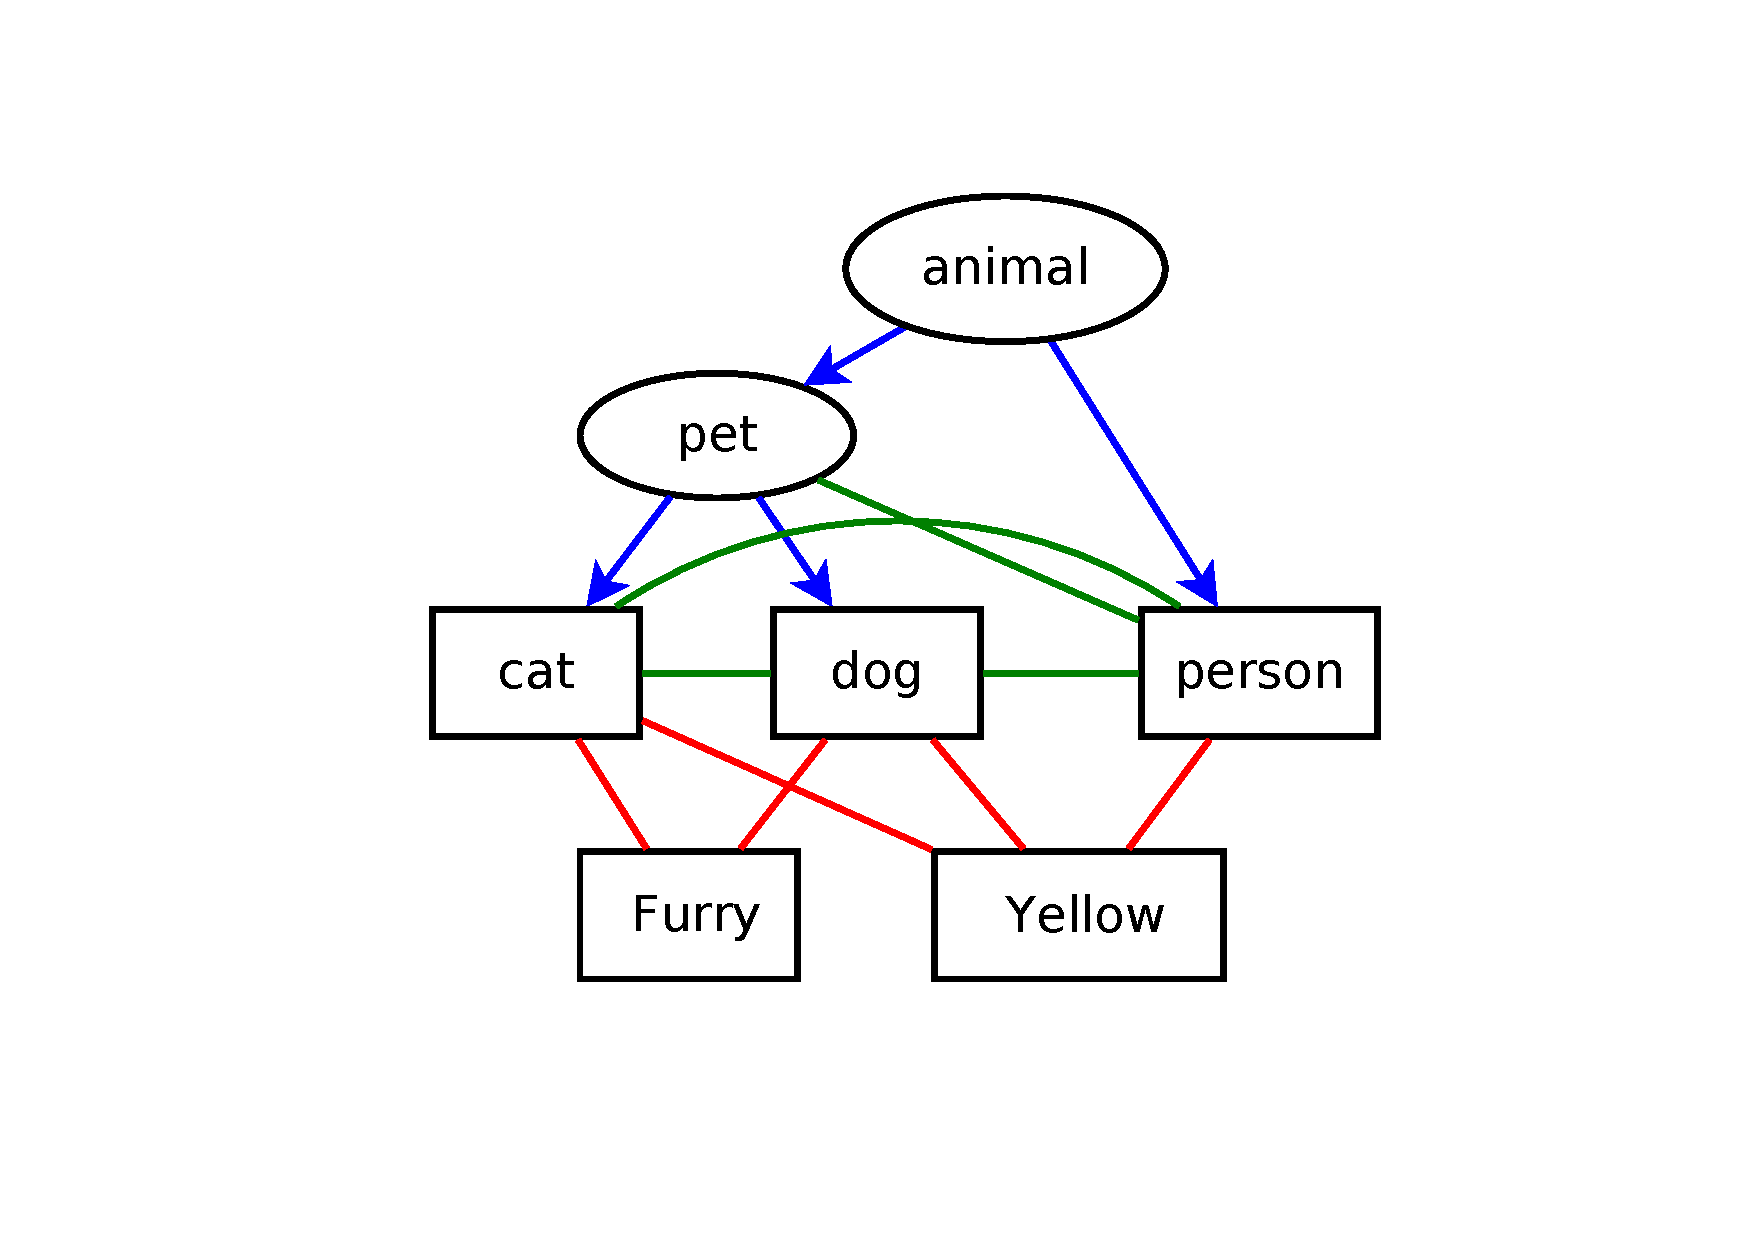
\includegraphics[scale=0.5]{ahex.pdf}
\caption{Attributed}
\label{fig:ahex}
\end{figure}

While the training data is provided by aPascal \& aYahoo dataset \cite{farhadi2009describing}. [TODO: discuss dataset properties] The possibility of using CNN as feature extractor has been confirmed in \cite{razavian2014cnn}.

We only connected attributes to bottom-level concepts. In other words, the aHEX graph can be seen as a semantic part and an attribute part. Such design is for the sake of reducing loops in the aHEX graph. While junction-tree algorithm could potentially handle such a loopy graph during inference stage, the loops makes the graph very tricky to learn as a CRF. Similar design has been applied to pixel labelling problem such as [TODO: find references].

However, it was not the loops that caused such idea to be dropped. Under the same non-learning model, potential function is submodular, therefore such extension s trivial. Under the learnable CRF model, the aHEX graph can be learned part-wise: the semantic subgraph can be learned in the same way as discussed in [TODO: cross-ref learnable CRF], whereas for the attributes part, all bottom-level concepts can be grouped into a super-concept with 20 states (corresponding to 20 PASCAL labels), then the attribute graph becomes a tree, which is learnable[TODO: find references]. With such model, the inference is the same as an non-learning system, as the potential function for the attributed part still has a submodular structure.

\section{Experiments with SVM as Underlying Unary Classifier}
\label{sec:svm}

\begin{table}[htbp]
\centering
\begin{tabular}{r|c|c|c}
 & 0\% & 50\% & 90\%\\
\hline
CNN Softmax  & 0.6698(0.8580) & 0.3325(0.7161) & 0.0112(0.5635)\\
Independent  & 0.1514(0.7226) & 0.0142(0.5540) & 0.0000(0.3147)\\
Original HEX & 0.6300(0.7612) & 0.2761(0.6846) & 0.0083(0.5754)\\
Stage 1      & 0.6300(0.7612) & 0.2761(0.6846) & 0.0083(0.5813)\\
Stage 2      & 0.6947(0.8010) & 0.4982(0.7523) & 0.1235(0.6781)\\
Stage 3      & 0.6692(0.7678) & 0.4530(0.6371) & 0.1597(0.4691)\\
\hline
Independent  & 0.7523(0.8990) & 0.6989(0.8711) & 0.4946(0.6882)\\
Original HEX & 0.7416(0.8812) & 0.7096(0.8515) & 0.5861(0.8117)\\
Stage 1      & 0.7399(0.8770) & 0.7090(0.8456) & 0.5855(0.8117)\\
Stage 2      & 0.6840(0.8491) & 0.5671(0.8176) & 0.4168(0.7553)
\end{tabular}
\caption{Comparison of empirical test result of different variants of the 	HEX model (rows) under different relabelling rates (columns), in the extended state space (upper) and the original one (lower). Performance is reported in accuracy, with top-3 accuracy in the bracket. Note that since the SVM array is naturally an independent multiclass classifier, CNN softmax is kept the a baseline.}
\label{tab:svmacc}
\end{table}

\begin{table}[htbp]
\centering
\begin{tabular}{r|c|c|c|c|c|c}
Concept & \makecell{CNN\\Softmax} & \makecell{Original\\HEX} & Stage 2 & Stage 3 & \makecell{Stage 2$-$\\Original} & \makecell{Stage 3$-$\\Stage 2}\\\hline
diningtable   & 0.4821 & 0.6250 & 0.7142 & 0.6964 & 0.0892 & -0.0178\\
chair         & 0.4666 & 0.2222 & 0.2666 & 0.2666 & 0.0444 & 0.0000\\
sofa          & 0.4310 & 0.3275 & 0.4137 & 0.3793 & 0.0862 & -0.0344\\
bottle        & 0.6000 & 0.4333 & 0.4666 & 0.4666 & 0.0333 & 0.0000\\
pottedplant   & 0.3928 & 0.4285 & 0.4642 & 0.4285 & 0.0357 & -0.0357\\
tvmonitor     & 0.8500 & 0.5500 & 0.5750 & 0.6000 & 0.0250 & 0.0250\\
train         & 0.8166 & 0.7333 & 0.8000 & 0.7583 & 0.0667 & -0.0417\\
bus           & 0.6764 & 0.6470 & 0.6911 & 0.7794 & 0.0441 & 0.0883\\
car           & 0.8281 & 0.6640 & 0.7343 & 0.6953 & 0.0703 & -0.0390\\
bicycle       & 0.8148 & 0.7037 & 0.7407 & 0.7962 & 0.0370 & 0.0555\\
motorbike     & 0.8035 & 0.6607 & 0.7500 & 0.6964 & 0.0893 & -0.0536\\
aeroplane     & 0.8137 & 0.7862 & 0.8413 & 0.8000 & 0.0551 & -0.0413\\
boat          & 0.6301 & 0.6712 & 0.6986 & 0.6575 & 0.0274 & -0.0411\\
cow           & 0.3269 & 0.4230 & 0.5576 & 0.4230 & 0.1346 & -0.1346\\
horse         & 0.4057 & 0.3188 & 0.4782 & 0.5072 & 0.1594 & 0.0290\\
sheep         & 0.3529 & 0.5588 & 0.5882 & 0.6176 & 0.0294 & 0.0294\\
dog           & 0.7272 & 0.6988 & 0.7272 & 0.7329 & 0.0284 & 0.0057\\
cat           & 0.5793 & 0.6896 & 0.7448 & 0.6896 & 0.0552 & -0.0552\\
bird          & 0.6886 & 0.8113 & 0.8679 & 0.8679 & 0.0566 & 0.0000\\
person        & 0.7313 & 0.6119 & 0.7064 & 0.6268 & 0.0945 & -0.0796\\\hline
household     & N/A    & 0.7431 & 0.7431 & 0.7237 & 0.0000 & -0.0194\\
furniture     & N/A    & 0.6226 & 0.6729 & 0.6415 & 0.0503 & -0.0314\\
transport     & N/A    & 0.9208 & 0.9223 & 0.9192 & 0.0015 & -0.0031\\
landtransport & N/A    & 0.8591 & 0.8896 & 0.8920 & 0.0305 & 0.0024\\
animal        & N/A    & 0.9195 & 0.9284 & 0.9208 & 0.0089 & -0.0076\\
livestock     & N/A    & 0.5677 & 0.6516 & 0.6451 & 0.0839 & -0.0065\\
pet           & N/A    & 0.8641 & 0.9039 & 0.9016 & 0.0398 & -0.0023
\end{tabular}
\caption{Comparison of accuracy broken down to concepts, under 0\% relabelling rate, in the extended state space, with SVM as the underlying unary classifier.}
\label{tab:svm0acc}
\end{table}

\begin{table}[htbp]
\centering
\begin{tabular}{r|c|c|c|c|c|c}
Concept & \makecell{CNN\\Softmax} & \makecell{Original\\HEX} & Stage 2 & Stage 3 & \makecell{Stage 2$-$\\Original} & \makecell{Stage 3$-$\\Stage 2}\\\hline
diningtable   & 0.2321 & 0.3214 & 0.6428 & 0.5357 & 0.3214 & -0.1071\\
chair         & 0.0888 & 0.0222 & 0.1333 & 0.1333 & 0.1111 & 0.0000\\
sofa          & 0.1206 & 0.0689 & 0.1896 & 0.1379 & 0.1207 & -0.0517\\
bottle        & 0.3000 & 0.1333 & 0.3333 & 0.3666 & 0.2000 & 0.0333\\
pottedplant   & 0.1071 & 0.1785 & 0.4285 & 0.3928 & 0.2500 & -0.0357\\
tvmonitor     & 0.5250 & 0.3000 & 0.4750 & 0.5250 & 0.1750 & 0.0500\\
train         & 0.1583 & 0.3416 & 0.5583 & 0.4333 & 0.2167 & -0.1250\\
bus           & 0.0294 & 0.3088 & 0.5441 & 0.7647 & 0.2353 & 0.2206\\
car           & 0.0703 & 0.2500 & 0.4687 & 0.3359 & 0.2187 & -0.1328\\
bicycle       & 0.1481 & 0.2407 & 0.5370 & 0.8148 & 0.2963 & 0.2778\\
motorbike     & 0.3214 & 0.2857 & 0.4821 & 0.3571 & 0.1964 & -0.1250\\
aeroplane     & 0.5034 & 0.3517 & 0.6137 & 0.5034 & 0.2620 & -0.1103\\
boat          & 0.2602 & 0.2054 & 0.5068 & 0.4109 & 0.3014 & -0.0959\\
cow           & 0.1153 & 0.1153 & 0.4038 & 0.2115 & 0.2885 & -0.1923\\
horse         & 0.1304 & 0.1594 & 0.3333 & 0.5507 & 0.1739 & 0.2174\\
sheep         & 0.2352 & 0.2352 & 0.4705 & 0.5882 & 0.2353 & 0.1177\\
dog           & 0.6363 & 0.3181 & 0.5170 & 0.4147 & 0.1989 & -0.1023\\
cat           & 0.4137 & 0.3241 & 0.5448 & 0.4620 & 0.2207 & -0.0828\\
bird          & 0.5000 & 0.3584 & 0.6603 & 0.6603 & 0.3019 & 0.0000\\
person        & 0.5373 & 0.3283 & 0.4925 & 0.4129 & 0.1642 & -0.0796\\\hline
household     & N/A    & 0.7548 & 0.7509 & 0.7237 & -0.0039 & -0.0272\\
furniture     & N/A    & 0.6289 & 0.7106 & 0.6477 & 0.0817 & -0.0629\\
transport     & N/A    & 0.9177 & 0.9208 & 0.9192 & 0.0031 & -0.0016\\
landtransport & N/A    & 0.8521 & 0.8943 & 0.8967 & 0.0422 & 0.0024\\
animal        & N/A    & 0.9118 & 0.9195 & 0.9144 & 0.0077 & -0.0051\\
livestock     & N/A    & 0.5935 & 0.6838 & 0.6451 & 0.0903 & -0.0387\\
pet           & N/A    & 0.8477 & 0.8922 & 0.8969 & 0.0445 & 0.0047
\end{tabular}
\caption{Comparison of accuracy broken down to concepts, under 50\% relabelling rate, in the extended state space, with SVM as the underlying unary classifier.}
\label{tab:svm50acc}
\end{table}

\begin{table}[htbp]
\centering
\begin{tabular}{r|c|c|c|c|c|c}
Concept & \makecell{CNN\\Softmax} & \makecell{Original\\HEX} & Stage 2 & Stage 3 & \makecell{Stage 2$-$\\Original} & \makecell{Stage 3$-$\\Stage 2}\\\hline
diningtable   & 0.0000 & 0.0000 & 0.2678 & 0.0892 & 0.2678 & -0.1786\\
chair         & 0.0000 & 0.0000 & 0.0222 & 0.0222 & 0.0222 & 0.0000\\
sofa          & 0.0000 & 0.0000 & 0.0172 & 0.0000 & 0.0172 & -0.0172\\
bottle        & 0.0000 & 0.0000 & 0.0333 & 0.0333 & 0.0333 & 0.0000\\
pottedplant   & 0.0000 & 0.0357 & 0.1428 & 0.2142 & 0.1071 & 0.0714\\
tvmonitor     & 0.0000 & 0.0250 & 0.0750 & 0.2000 & 0.0500 & 0.1250\\
train         & 0.0083 & 0.0083 & 0.1916 & 0.0250 & 0.1833 & -0.1666\\
bus           & 0.0147 & 0.0147 & 0.1911 & 0.7647 & 0.1764 & 0.5736\\
car           & 0.0000 & 0.0000 & 0.1250 & 0.0312 & 0.1250 & -0.0938\\
bicycle       & 0.0000 & 0.0000 & 0.1851 & 0.8518 & 0.1851 & 0.6667\\
motorbike     & 0.0000 & 0.0000 & 0.0714 & 0.0178 & 0.0714 & -0.0536\\
aeroplane     & 0.0137 & 0.0068 & 0.1172 & 0.0344 & 0.1104 & -0.0828\\
boat          & 0.0000 & 0.0000 & 0.1232 & 0.0684 & 0.1232 & -0.0548\\
cow           & 0.0192 & 0.0000 & 0.0384 & 0.0000 & 0.0384 & -0.0384\\
horse         & 0.0144 & 0.0000 & 0.0289 & 0.4637 & 0.0289 & 0.4348\\
sheep         & 0.0000 & 0.0000 & 0.0588 & 0.5294 & 0.0588 & 0.4706\\
dog           & 0.0397 & 0.0056 & 0.1477 & 0.0625 & 0.1421 & -0.0852\\
cat           & 0.0000 & 0.0344 & 0.1517 & 0.0758 & 0.1173 & -0.0759\\
bird          & 0.0188 & 0.0094 & 0.1792 & 0.1698 & 0.1698 & -0.0094\\
person        & 0.0199 & 0.0099 & 0.0895 & 0.0447 & 0.0796 & -0.0448\\\hline
household     & N/A    & 0.7509 & 0.7431 & 0.7081 & -0.0078 & -0.0350\\
furniture     & N/A    & 0.6226 & 0.7044 & 0.6352 & 0.0818 & -0.0692\\
transport     & N/A    & 0.9177 & 0.9192 & 0.9192 & 0.0015 & 0.0000\\
landtransport & N/A    & 0.8521 & 0.8967 & 0.8896 & 0.0446 & -0.0071\\
animal        & N/A    & 0.9093 & 0.9080 & 0.9118 & -0.0013 & 0.0038\\
livestock     & N/A    & 0.5870 & 0.6838 & 0.6838 & 0.0968 & 0.0000\\
pet           & N/A    & 0.8384 & 0.8922 & 0.8899 & 0.0538 & -0.0023
\end{tabular}
\caption{Comparison of accuracy broken down to concepts, under 90\% relabelling rate, in the extended state space, with SVM as the underlying unary classifier.}
\label{tab:svm90acc}
\end{table}

\begin{table}[htbp]
\centering
\begin{tabular}{r|c|c|c}
Concept & 0\% & 50\% & 90\%\\\hline
diningtable   & $0.4804\pm0.1966$ & $0.3840\pm0.1581$ & $0.2409\pm0.0641$\\
chair         & $0.3722\pm0.1553$ & $0.3001\pm0.1167$ & $0.2227\pm0.0789$\\
sofa          & $0.4534\pm0.2143$ & $0.3379\pm0.1419$ & $0.2337\pm0.0793$\\
bottle        & $0.5479\pm0.2583$ & $0.3764\pm0.1434$ & $0.2797\pm0.1136$\\
pottedplant   & $0.4661\pm0.2345$ & $0.3604\pm0.1689$ & $0.2582\pm0.0950$\\
tvmonitor     & $0.5667\pm0.2350$ & $0.4103\pm0.1913$ & $0.2304\pm0.0936$\\
train         & $0.7275\pm0.2600$ & $0.4189\pm0.1779$ & $0.2538\pm0.0853$\\
bus           & $0.7250\pm0.1979$ & $0.4219\pm0.1837$ & $0.2560\pm0.0800$\\
car           & $0.6404\pm0.2816$ & $0.3763\pm0.1844$ & $0.2469\pm0.0846$\\
bicycle       & $0.6018\pm0.2739$ & $0.4036\pm0.1604$ & $0.2349\pm0.0751$\\
motorbike     & $0.5953\pm0.2172$ & $0.4035\pm0.1642$ & $0.2171\pm0.1010$\\
aeroplane     & $0.7229\pm0.2358$ & $0.4251\pm0.1835$ & $0.2362\pm0.1036$\\
boat          & $0.6580\pm0.2325$ & $0.4247\pm0.2081$ & $0.2646\pm0.0903$\\
cow           & $0.4227\pm0.1850$ & $0.3146\pm0.1479$ & $0.2227\pm0.0634$\\
horse         & $0.5085\pm0.2165$ & $0.3735\pm0.1467$ & $0.2220\pm0.0736$\\
sheep         & $0.4951\pm0.1858$ & $0.3590\pm0.1482$ & $0.2332\pm0.0900$\\
dog           & $0.6190\pm0.2490$ & $0.4123\pm0.1935$ & $0.2568\pm0.1072$\\
cat           & $0.6688\pm0.2459$ & $0.4223\pm0.1796$ & $0.2707\pm0.1041$\\
bird          & $0.7018\pm0.2342$ & $0.4219\pm0.1795$ & $0.2703\pm0.1179$\\
person        & $0.5841\pm0.2590$ & $0.3971\pm0.2080$ & $0.2465\pm0.1077$\\\hline
household     & $0.6598\pm0.2280$ & $0.6598\pm0.2280$ & $0.6598\pm0.2280$\\
furniture     & $0.5707\pm0.2492$ & $0.5707\pm0.2492$ & $0.5707\pm0.2492$\\
transport     & $0.8052\pm0.1949$ & $0.8052\pm0.1949$ & $0.8052\pm0.1949$\\
landtransport & $0.7691\pm0.2267$ & $0.7691\pm0.2267$ & $0.7691\pm0.2267$\\
animal        & $0.7816\pm0.2167$ & $0.7816\pm0.2167$ & $0.7816\pm0.2167$\\
livestock     & $0.6098\pm0.2389$ & $0.6098\pm0.2389$ & $0.6098\pm0.2389$\\
pet           & $0.7394\pm0.2151$ & $0.7394\pm0.2151$ & $0.7394\pm0.2151$
\end{tabular}
\caption{Under different relabelling rates, with SVM as the underlying unary classifier, the mean and standard deviation of sigmoid-transformed response (distance to decision boundary) on validation images, broken down to concepts.}
\label{tab:svmresp}
\end{table}

\begin{table}[htbp]
\centering
\begin{tabular}{r|c|c|c|c}
Node & 0\% & 50\% & 90\% & 90\%$-$0\%\\\hline
diningtable   & 1.9265 & 1.9236 & 1.7988 & -0.1277\\
chair         & 1.3386 & 1.2640 & 1.2966 & -0.0420\\
sofa          & 1.8851 & 1.9036 & 1.8286 & -0.0565\\
bottle        & 0.6659 & 0.6271 & 0.8228 & 0.1569\\
pottedplant   & 0.9247 & 0.8957 & 0.9201 & -0.0046\\
tvmonitor     & 0.4994 & 0.7050 & 0.5832 & 0.0838\\
train         & 1.8813 & 1.9102 & 1.8070 & -0.0743\\
bus           & 0.0450 & 0.0297 & 0.0224 & -0.0226\\
car           & 0.9947 & 1.1058 & 0.9904 & -0.0043\\
bicycle       & 0.0000 & 0.0000 & 0.0000 & 0.0000\\
motorbike     & 1.9338 & 1.9510 & 1.9340 & 0.0002\\
aeroplane     & 1.8529 & 1.9190 & 1.8513 & -0.0016\\
boat          & 1.4451 & 1.5748 & 1.4387 & -0.0064\\
cow           & 1.4513 & 1.4529 & 1.3184 & -0.1329\\
horse         & 0.0000 & 0.0000 & 0.0220 & 0.0220\\
sheep         & 0.0000 & 0.0000 & 0.0000 & 0.0000\\
dog           & 1.7648 & 1.8041 & 1.7249 & -0.0399\\
cat           & 1.7568 & 1.8101 & 1.7346 & -0.0222\\
bird          & 3.5105 & 3.1755 & 3.2677 & -0.2428\\
person        & 1.2342 & 1.2741 & 1.2668 & 0.0326\\\hline
household     & 0.8339 & 0.9198 & 0.9864 & 0.1525\\
furniture     & 1.6695 & 1.6110 & 1.7586 & 0.0891\\
transport     & 0.4305 & 0.4510 & 1.0331 & 0.6026\\
landtransport & 2.6186 & 2.5675 & 2.9159 & 0.2973\\
animal        & 2.5923 & 2.4176 & 2.6773 & 0.0850\\
livestock     & 0.0000 & 0.0000 & 0.0000 & 0.0000\\
pet           & 3.8558 & 3.8488 & 3.9997 & 0.1439
\end{tabular}
\caption{Unary weights learned in stage 3, with SVM as the underlying classifier.}
\label{tab:svmunary}
\end{table}

\begin{table}[htbp]
\centering
\begin{tabular}{r|c|c|c|c}
Edge & 0\% & 50\% & 90\% & 90\%$-$0\%\\\hline
(household, bottle)        & 0.9506 & 0.9503 & 0.9371 & -0.0135\\
(household, pottedplant)   & 1.1450 & 1.1220 & 1.1862 & 0.0412\\
(household, tvmonitor)     & 0.9465 & 0.9477 & 0.9507 & 0.0042\\
(household, furniture)     & 0.6116 & 0.6318 & 0.6151 & 0.0035\\
(furniture, diningtable)   & 0.9365 & 0.9363 & 0.9276 & -0.0089\\
(furniture, chair)         & 0.9657 & 0.9668 & 0.9777 & 0.0120\\
(furniture, sofa)          & 0.9170 & 0.9223 & 0.9177 & 0.0007\\
(transport, aeroplane)     & 0.8285 & 0.8477 & 0.8472 & 0.0187\\
(transport, boat)          & 0.8906 & 0.8989 & 0.8841 & -0.0065\\
(transport, landtransport) & 2.0117 & 1.9375 & 2.0144 & 0.0027\\
(landtransport, train)     & 0.8558 & 0.8691 & 0.8663 & 0.0105\\
(landtransport, bus)       & 1.2733 & 1.2454 & 1.2599 & -0.0134\\
(landtransport, car)       & 0.9485 & 0.9586 & 1.0058 & 0.0573\\
(landtransport, bicycle)   & 1.0078 & 1.0127 & 1.0162 & 0.0084\\
(landtransport, motorbike) & 0.8892 & 0.8977 & 0.9047 & 0.0155\\
(animal, person)           & 0.9056 & 0.9143 & 0.8878 & -0.0178\\
(animal, livestock)        & 0.7380 & 0.7416 & 0.8540 & 0.1160\\
(animal, pet)              & 1.8121 & 1.8469 & 2.0426 & 0.2305\\
(livestock, cow)           & 0.9483 & 0.9517 & 0.9559 & 0.0076\\
(livestock, horse)         & 0.9648 & 0.9715 & 0.9677 & 0.0029\\
(livestock, sheep)         & 1.0186 & 1.0184 & 1.0406 & 0.0220\\
(pet, dog)                 & 0.8137 & 0.8258 & 0.8076 & -0.0061\\
(pet, cat)                 & 0.8031 & 0.8261 & 0.8021 & -0.0010\\
(pet, bird)                & 3.0280 & 2.8567 & 3.1028 & 0.0748
\end{tabular}
\caption{Pairwise weights learned in stage 3, with SVM as the underlying classifier.}
\label{tab:svmpairwise}
\end{table}

\clearpage
\bibliographystyle{plain}
\bibliography{ref}
\end{document}